\chapter{Microstructural Evaluation}
\label{chap:microstructure_eval}

\chaptertoc{}

\begin{chapterabstract}
  This chapter presents a series of experiments performed using \ac{ConFiG} phantoms to test their microstructural realism, something essential to prove the value of \ac{ConFiG} phantoms.

  Firstly, the methodology used to calculate microstructural features from \ac{ConFiG} phantom meshes are presented. The dependency of some of these features on the input morphology is demonstrated, followed by a series of experiments which compare \ac{ConFiG} phantoms to real white matter reconstructed from electron microscopy.
\end{chapterabstract}



\section{Introduction}
\label{sec:micro_introduction}
As demonstrated in \Cref{chap:config}, \ac{ConFiG} is able to generate \acf{WM} numerical phantoms which can be used to generate realistic simulated \acf{dMRI} signals. Whilst this a valuable check of the realism of the phantoms, this does not guarantee that the underlying microstructure is realistic since simplistic representations such as straight parallel cylinders can be used to generate realistic signals in certain cases.

To investigate how well axons generated using \ac{ConFiG} represent real \ac{WM} axons, a series of experiments were conducted to compare \ac{ConFiG} axons to real axons reconstructed from \acf{EM}. Typical \ac{EM} technqiues such as \acf{SEM} and \acf{TEM} provide only 2D images of tissue cross-sections, giving only limited information on axonal morphology. Recent technological improvements - primarily improvements and increased accessibility of \acf{SBEM}\cite{Helmstaedter2008,Denk2004}, a technique to take \ac{SEM} images of many sequential tissue slices - have enabled new possibilities for the study of axonal microstructure in 3D.

Although high-resolution 3D imaging of tissue is possible using these \ac{SBEM} techniques, segmentation and quantification of the resulting images has remained challenging, meaning that there have only been a few studies investigating the 3D microstructure of segmented axons in \ac{WM} \cite{Abdollahzadeh2019,Lee2019b,Salo2018}. Of these, only Lee et al.\ \cite{Lee2019b} have made their axonal segmentations publicly available so it is this data set that we use to compare with \ac{ConFiG}.

The rest of the chapter is arranged as follows, \Cref{sec:micro_measurements} describes the procedures used to extract microstructural features from the 3D meshes generated by \ac{ConFiG}.~\Cref{sec:micro_experiments} outlines a set of experiments that were performed using these microstructural measurement techniques to assess how the complexity of fibre arrangements affect the axonal morphology and to compare \ac{ConFiG} axons to real axons segmented from \ac{EM}. \Cref{sec:micro_results} presents the results of these experiments and \Cref{sec:micro_discussion} summarises the contributions and discusses future work.


\section{Microstructural measurements}
\label{sec:micro_measurements}

\begin{figure}
  \centering
  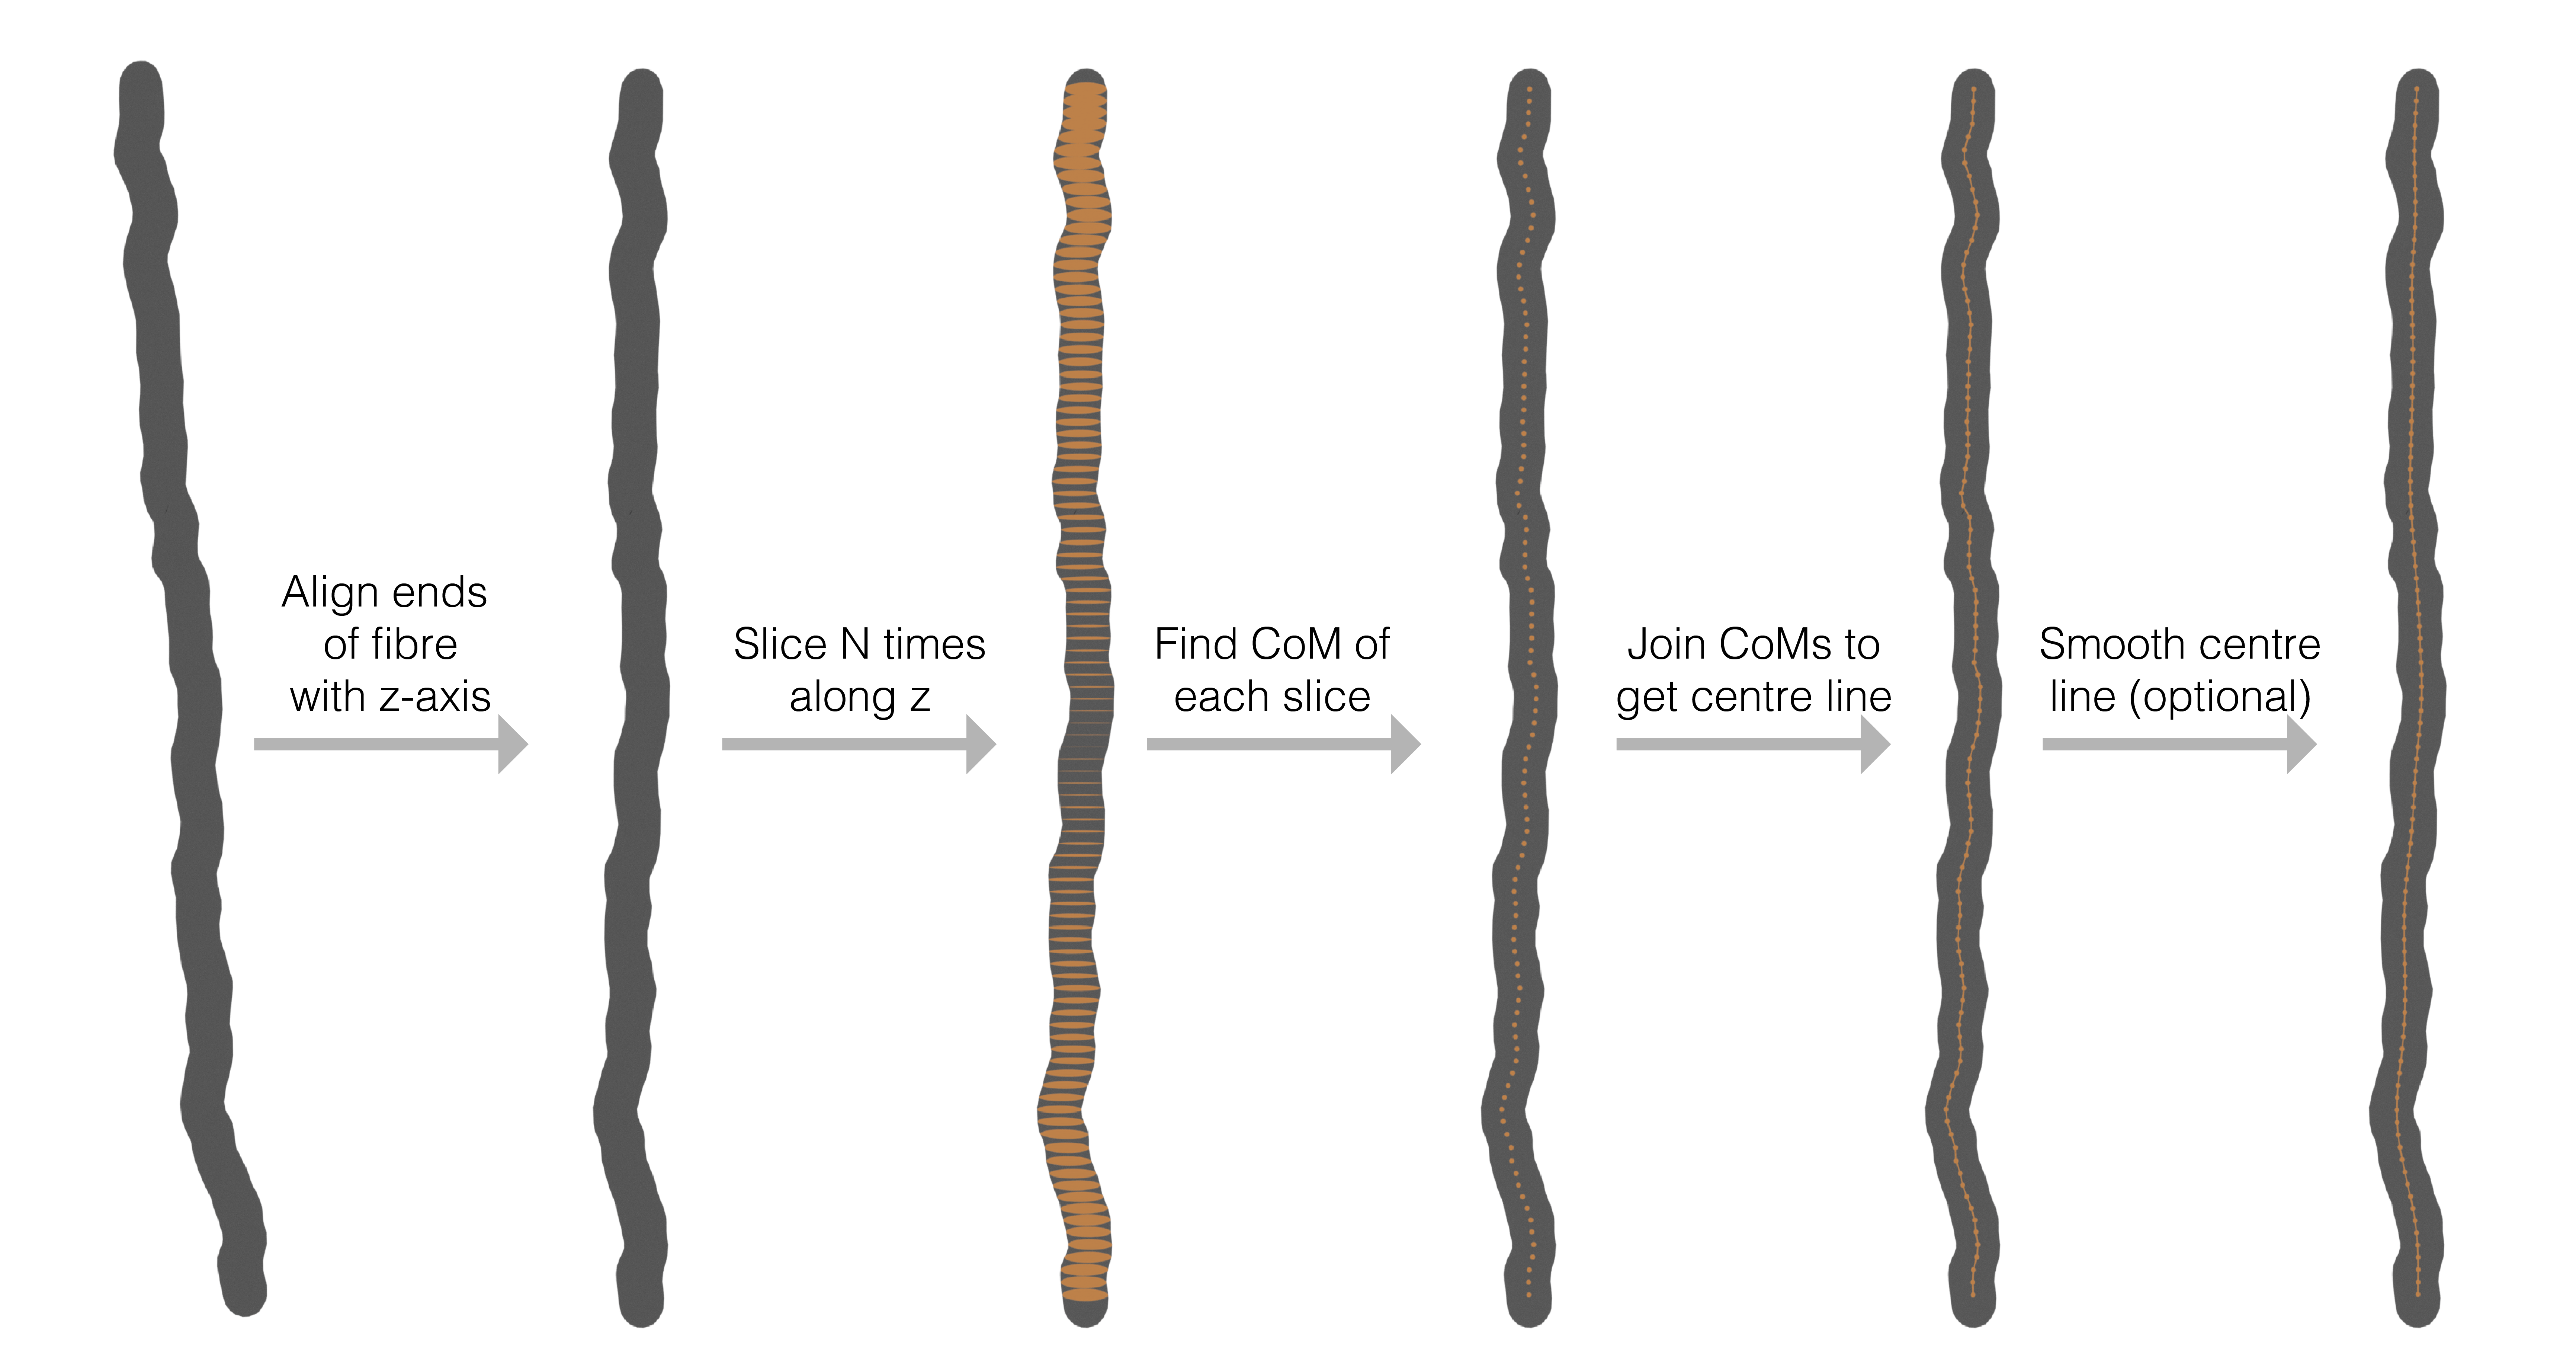
\includegraphics[width=\textwidth]{figures/config/centre_line_extraction-01.png}
  \caption[Mesh centreline extraction]{Centre line extraction of fibres. Each fibre was sliced N times along the z-axis, connecting the centre of mass of each slice to create the points in the centre line. This line could then be optionally smoothed according the diffusion time coarse graining effect, as in \cite{Lee2019b}}
  \label{fig:config_micro_centreline}
\end{figure}

In order to test how realistic the microstructure generated using \ac{ConFiG} is, microstructural measurements of diameter distribution and orientation distribution were calculated using methods to be comparable with previous studies on ex-vivo tissue \cite{Abdollahzadeh2019,Lee2019b}.

A centre line is generated from each of the fibre meshes by aligning the ends of each fibre with the z-axis and connecting the centre of mass of 100 equidistant slices through each fibre, following the approach taken by Lee et al., \cite{Lee2019b}. This is illustrated in \Cref{fig:config_micro_centreline}.

Each segment in this centre line could then be used to assess the microstructure of the phantom. The direction of each segment was used to assess the orientation distribution of the phantom, illustrated in \Cref{fig:config_micro_OD}. Following the approach of Lee et al., \cite{Lee2019b}, the direction of each segment was projected onto the surface of a triangulated unit sphere \cite{Womersley2018}. For each triangle, the number of segments pointing in that direction was used to colour the triangle to visualise the orientation distribution.

\begin{figure}
  \centering
  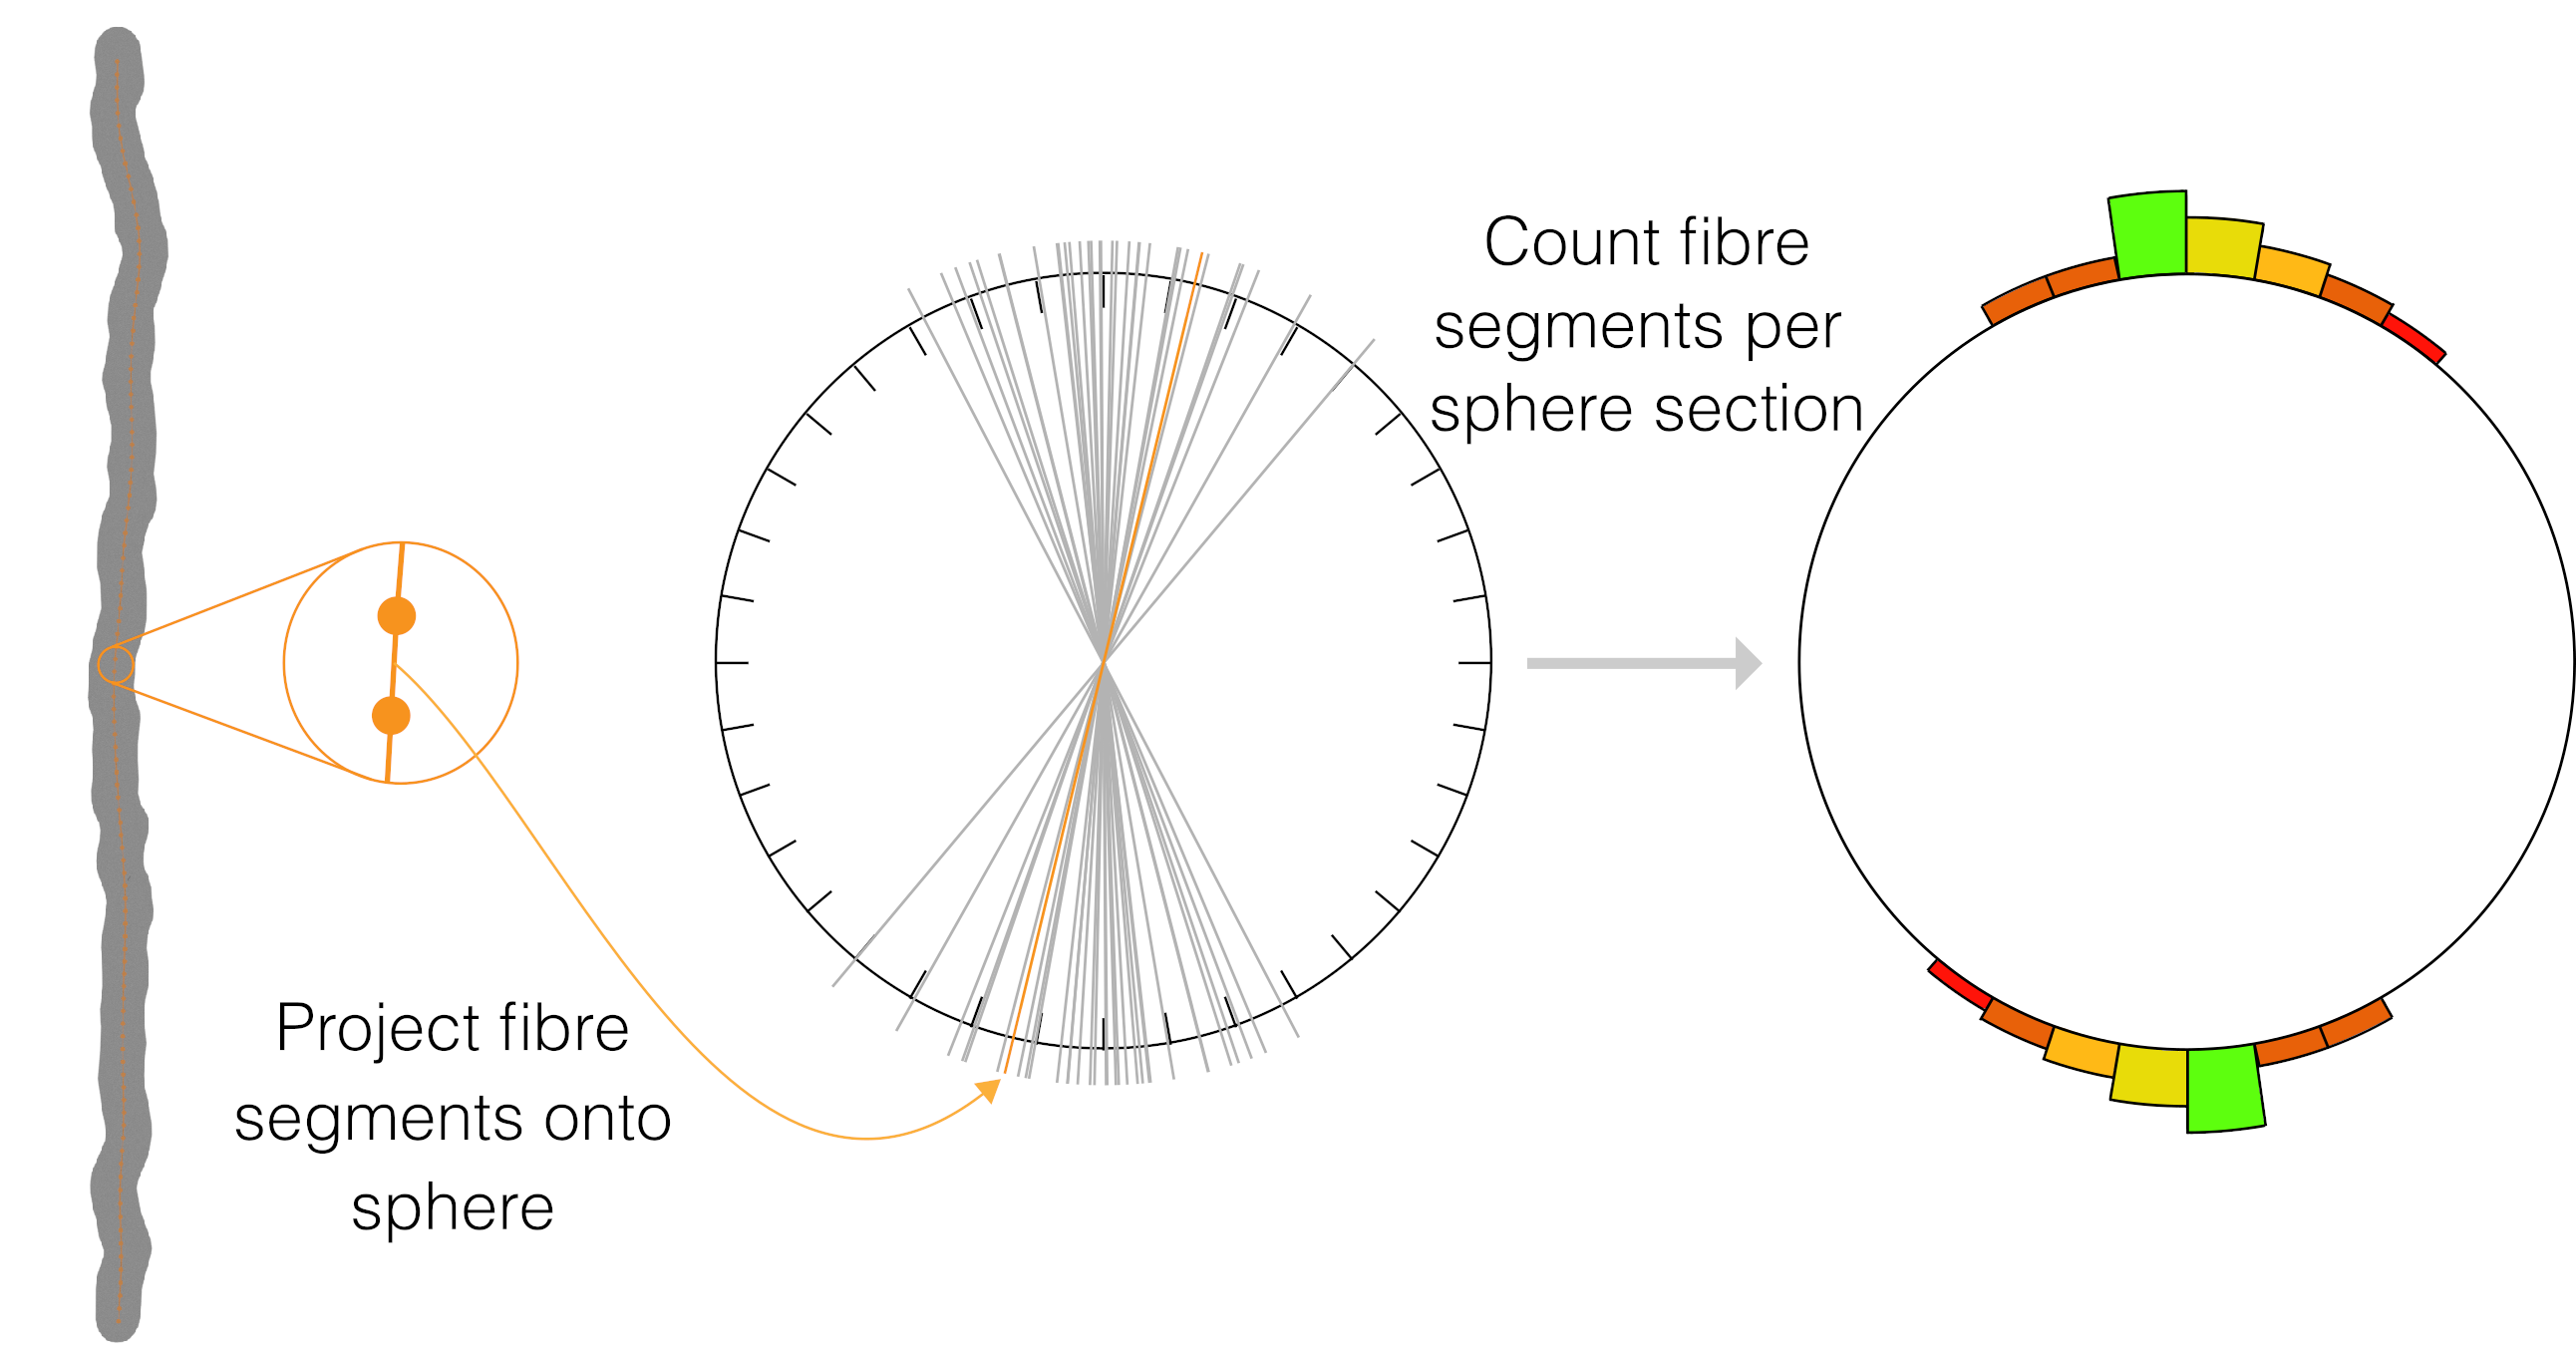
\includegraphics[width=\textwidth]{figures/config/od_calculation-01_sym_whitebg.png}
  \caption[Orientation distribution extraction from microstructure]{Orientation distribution calculation. Each segment of a fibre was projected onto the surface of a triangulated sphere, here illustrated with a sectioned circle. For each section in the sphere, the number of fibre segments going through that section was used to colour and/or raise the surface to visualise the orientation distribution. Since the diffusion process is symmetric about the origin, each fibre segment was projected onto the sphere forwards and backwards.}
  \label{fig:config_micro_OD}
\end{figure}

\begin{figure}
  \centering
  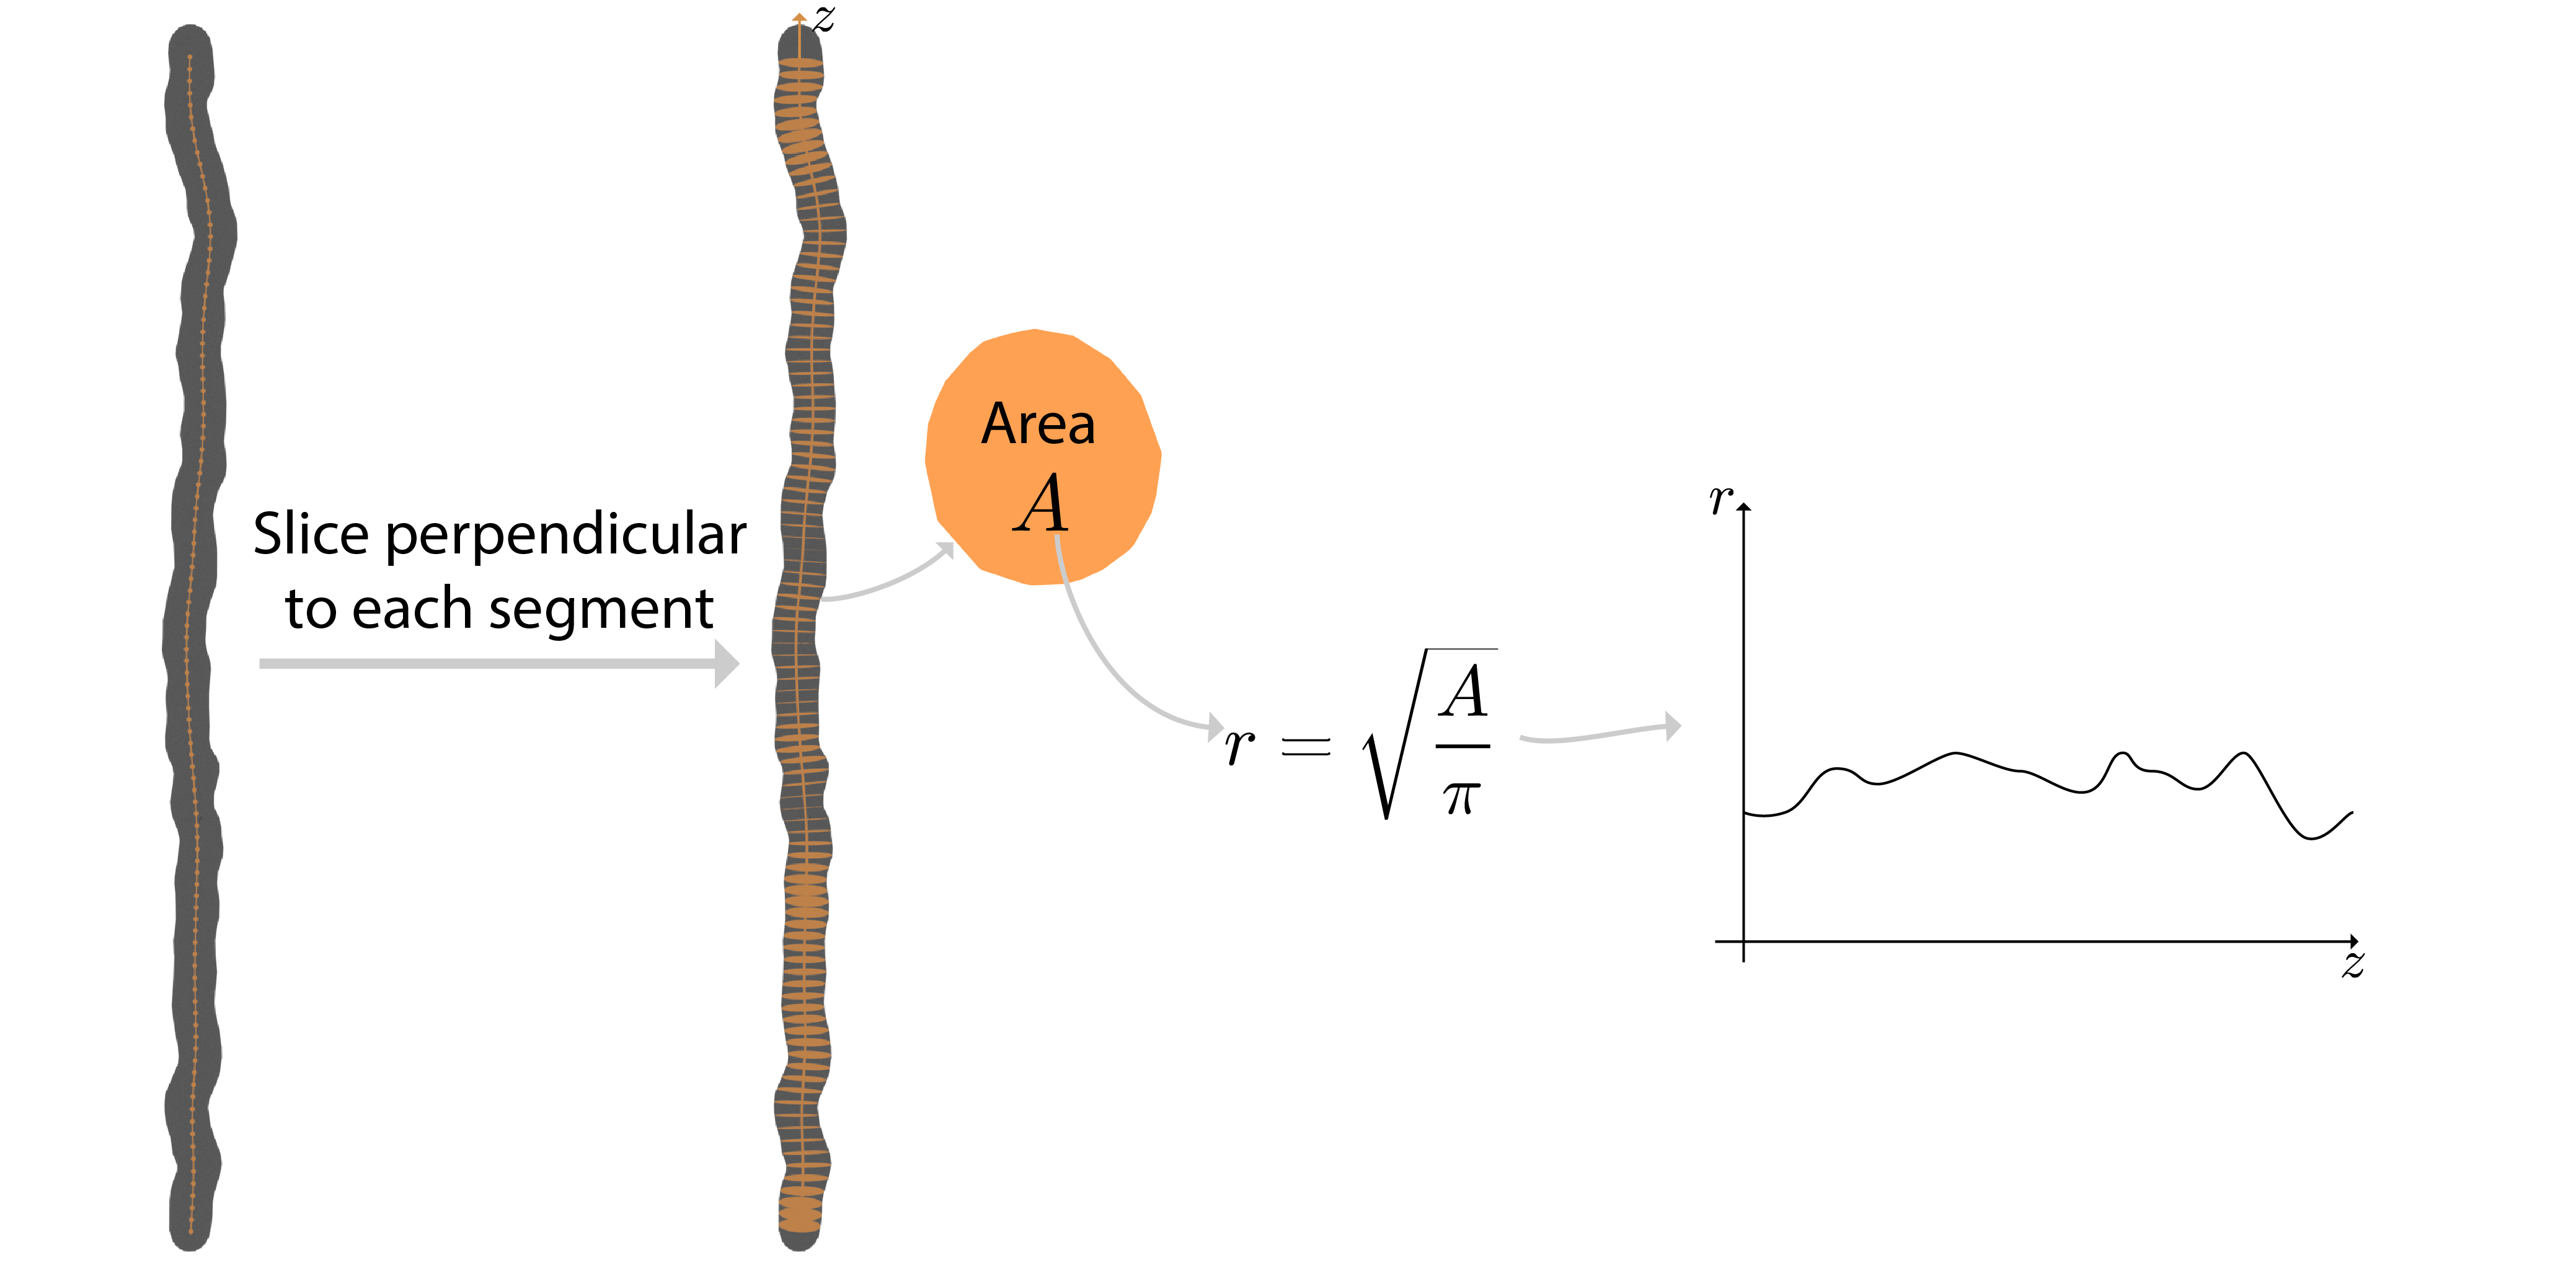
\includegraphics[width=\textwidth]{figures/config/diam_calculation-01.png}
  \caption[Diameter distribution extraction from microstructure]{Calculation of the diameter distribution. A slice is taken through each fibre perpendicular to every segment in the centre line. The area of each of these slices is used to find a circle equivalent radius or diameter using $A = \pi r^2$. }
  \label{fig:config_micro_diam}
\end{figure}

A second approach was devised to better visualise orientation distributions in 3D to aid differentiation of crossing bundles and antipodal symmetry. In this approach each vertex was raised above the surface of the sphere proportionally to the number of segments pointing in its direction as illustrated in \Cref{fig:config_micro_OD}.

To measure the diameter profile along fibres, the direction of each segment gave the normal to a plane used to cut the fibre using Boolean intersection to give a cross section of each fibre at each segment. The diameter profile along the axon was generated by calculating the equivalent diameter of a circle with the same area as the fibre cross section. This process is illustrated in \Cref{fig:config_micro_diam}.

\subsection{Virtual histology and 2D morphological measures}
\label{sec:confg_virtual_histology}
Virtual histological slices were generated to compare \ac{ConFiG} substrates to real white matter analysed using histology. Histological slices were found by calculating the Boolean intersection of a cutting plane with the generated fibre meshes using Blender (\url{https://blender.org}). A myelin sheath was added to the fibres when generating virtual histology for visualisation purposes.  Virtual histological images were rendered with a resolution of \SI{5 x 5 x 100}{\nano\metre}, chosen to be comparable to real histological white matter measurements \cite{Abdollahzadeh2019,Lee2019b}.

In order to compare \ac{ConFiG} virtual histology to real histology, virtual histological slices were rendered in binary black and white to compare against intra-axonal segmentations from \cite{Lee2019b}. Slices from real histology, \ac{ConFiG} phantoms and a parallel cylinder phantom were processed using the MorphoLibJ plugin for ImageJ \cite{Rueden2017,Legland2016,Schindelin2012,Schneider2012} to extract morphological features: circularity ($4\pi$ × Area/Perimeter$^2$), convexity (Area of shape/Area of convex hull), eccentricity of fitted ellipse and Area/$\pi r_{max}^2$ for each axon. Axons touching the edge of the image were removed since truncation from the image edge would skew these microstructural metrics.

\section{Experiments}
\label{sec:micro_experiments}

\subsection{Relationship between input and output morphology}
\label{sec:config_input_output_rel}
As mentioned in \Cref{sec:config_methods}, the nature of the \ac{ConFiG} growth algorithm means that the microstructural morphology of the phantoms may not match the user input. Some fibres may become stuck and fibres cannot typically grow in a straight line, affecting the density and orientation distribution.

To investigate this, we generated a series of \ac{ConFiG} phantoms with Watson distributed \cite{Mardia2008} orientation dispersion with $\kappa=[8,10,15,20,30,50,100]$ and target density, $\rho = 75$\%. The target density of 75\% is chosen as this is the upper limit of what is achievable empirically and towards the higher end of expected axonal volume fraction. Additionally, with 75\% achieved, lower densities can be generated easily, either by running \ac{ConFiG} in full, or simply by removing or shrinking fibres.

The mean and standard deviation of the angle from $z$, $\mu_\theta$ and $\sigma_\theta$ respectively, for each $\kappa$ was calculated by taking $10000$ samples from the Watson distribution and this was compared to $\mu_\theta$ and $\sigma_\theta$ of the \ac{ConFiG} fibres. Additionally, the density of the \ac{ConFiG} phantoms was compared to the target density of 75\%. Each phantom was generated in a \SI{20 x 20 x 20}{\micro\metre} region, using \num{2.5e6} nodes in the growth network.

\subsection{Packing induced microsctructural complexity}
\label{sec:micro_packing_induced_complexity}
When axons grow, they must bend and bulge to grow around one another without colliding. It is a reasonable assumption to make that the level of divergence from straight cylinders is higher in more complex arrangements of fibres (i.e. in complex fibre arrangements such as high orientation dispersion, fibres are more likely to cross paths and so are more likely to need to deform around one another).

In order to test whether this effect is present in \ac{ConFiG} phantoms, we used the phantoms from \Cref{sec:config_input_output_rel}, with the addition of two phantoms generated with target $\kappa$ of 2 and 4 to attempt to generate even more complex arrangements. Each of these phantoms were generated with fibres that attempted to go straight from start to target point with a constant radius, so any deviations arise from the growth procedure itself rather than input settings.

For each fibre, the centreline was extracted as described in \Cref{sec:micro_measurements} and the end points of each fibre were used to calculate $\sigma_\theta$ for the fibres if they were joined by straight lines.
This is used as a proxy for the complexity of the phantom since a higher $\sigma_\theta$ will lead to more fibres crossing one another.
Additionally, for each phantom, the coefficient of variation of the diameter along each fibre was calculated as a measure of the amount of fibre beading and the tortuosity for each fibre was calculated as $\tau=L_{\mathrm{fibre}}/L_{\mathrm{ends}}$, the ratio of the total length of the fibre and the length of the straight line between endpoints.



\section{Results}
\label{sec:micro_results}

\subsection{Microstructural measures and virtual histology}
\label{sec:config_result_micro_meas}

\begin{figure}
  \centering
  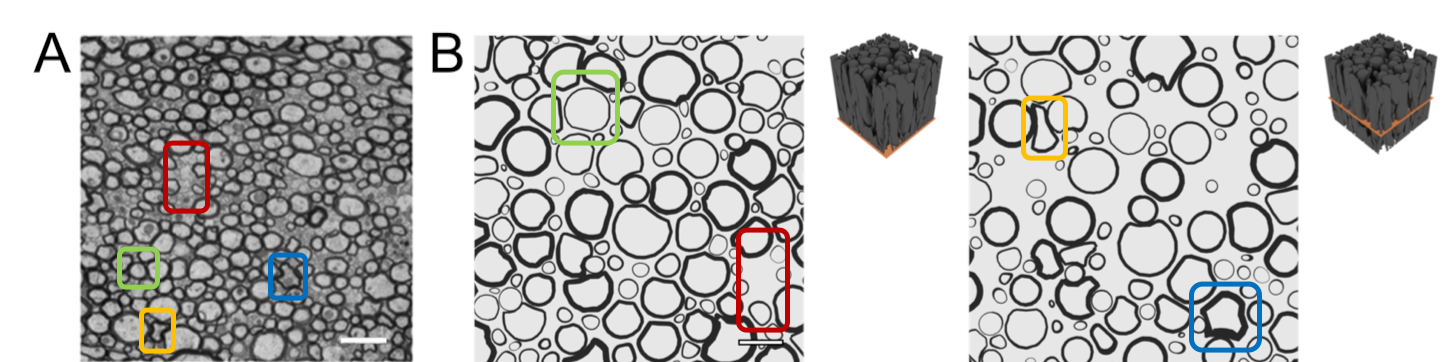
\includegraphics[width=\textwidth]{figures/config/virthist1_wbox_whitebg.png}
  \caption[Comparison of real and virtual histology]{Comparison of real  and virtual histology. A) Light microscopy of rat ventromedial WM in thoracic spinal cord. Reproduced from Baxi et al. 2015 (Baxi et al., 2015), scale bar 2microm. B) Two virtual histological slices from a \ac{ConFiG} generated phantom. Phantoms are rendered to have similar col ours to electron microscopy studies. The exact contrast and fibre bundle configurations are different between the real and virtual tissues, but the general morphology of the myelinated axons are captured well using \ac{ConFiG} as highlighted by corresponding boxes. Yellow and Blue: axons severely deformed between other axons. Red: Pockets of empty space forming. Green: Largely circular axon surrounded by other axons deforming around it. Scale bar 2microm.}
  \label{fig:config_res_real_vs_virt_hist}
\end{figure}

The microstructural morphology generated using \ac{ConFiG} is comparable to results from real data as demonstrated in \Cref{fig:config_res_real_vs_virt_hist,fig:config_res_slice_wise_metrics,fig:config_res_diameter_dist,fig:config_res_OD}.~\Cref{fig:config_res_real_vs_virt_hist} demonstrates virtual histology of a \ac{ConFiG} phantom alongside a real \ac{EM} image from mouse corpus callosum \cite{Baxi2015}. The exact microstructural features, such as diameter distribution, as well as the \ac{EM} contrast do not exactly match between \ac{ConFiG} and the real data. However, \ac{ConFiG} is able to capture the general morphology or real axons as highlighted in \Cref{fig:config_res_slice_wise_metrics,fig:config_res_diameter_dist}. In particular, \ac{ConFiG} is able to capture complex fibre cross-sections such as in the case of fibres squashed into small spaces. This is the first model of white matter able to handle complex fibre cross-sections such as this to our knowledge.

\ac{ConFiG} morphological metrics calculated slice-wise on the virtual histology correspond much more closely to real axons than the same metrics calculated for parallel cylinders, as shown in \Cref{fig:config_res_slice_wise_metrics}. While cylinders produce a delta function at one extreme of each metric, \ac{ConFiG} phantoms produce much closer distributions to the real data.~\Cref{fig:micro_slice_wise_colormap} shows each of these slices coloured by their morphological metrics, demonstrating which fibres are contributing to the distributions of each metric shown in \Cref{fig:config_res_slice_wise_metrics}.

\begin{figure}
  \centering
  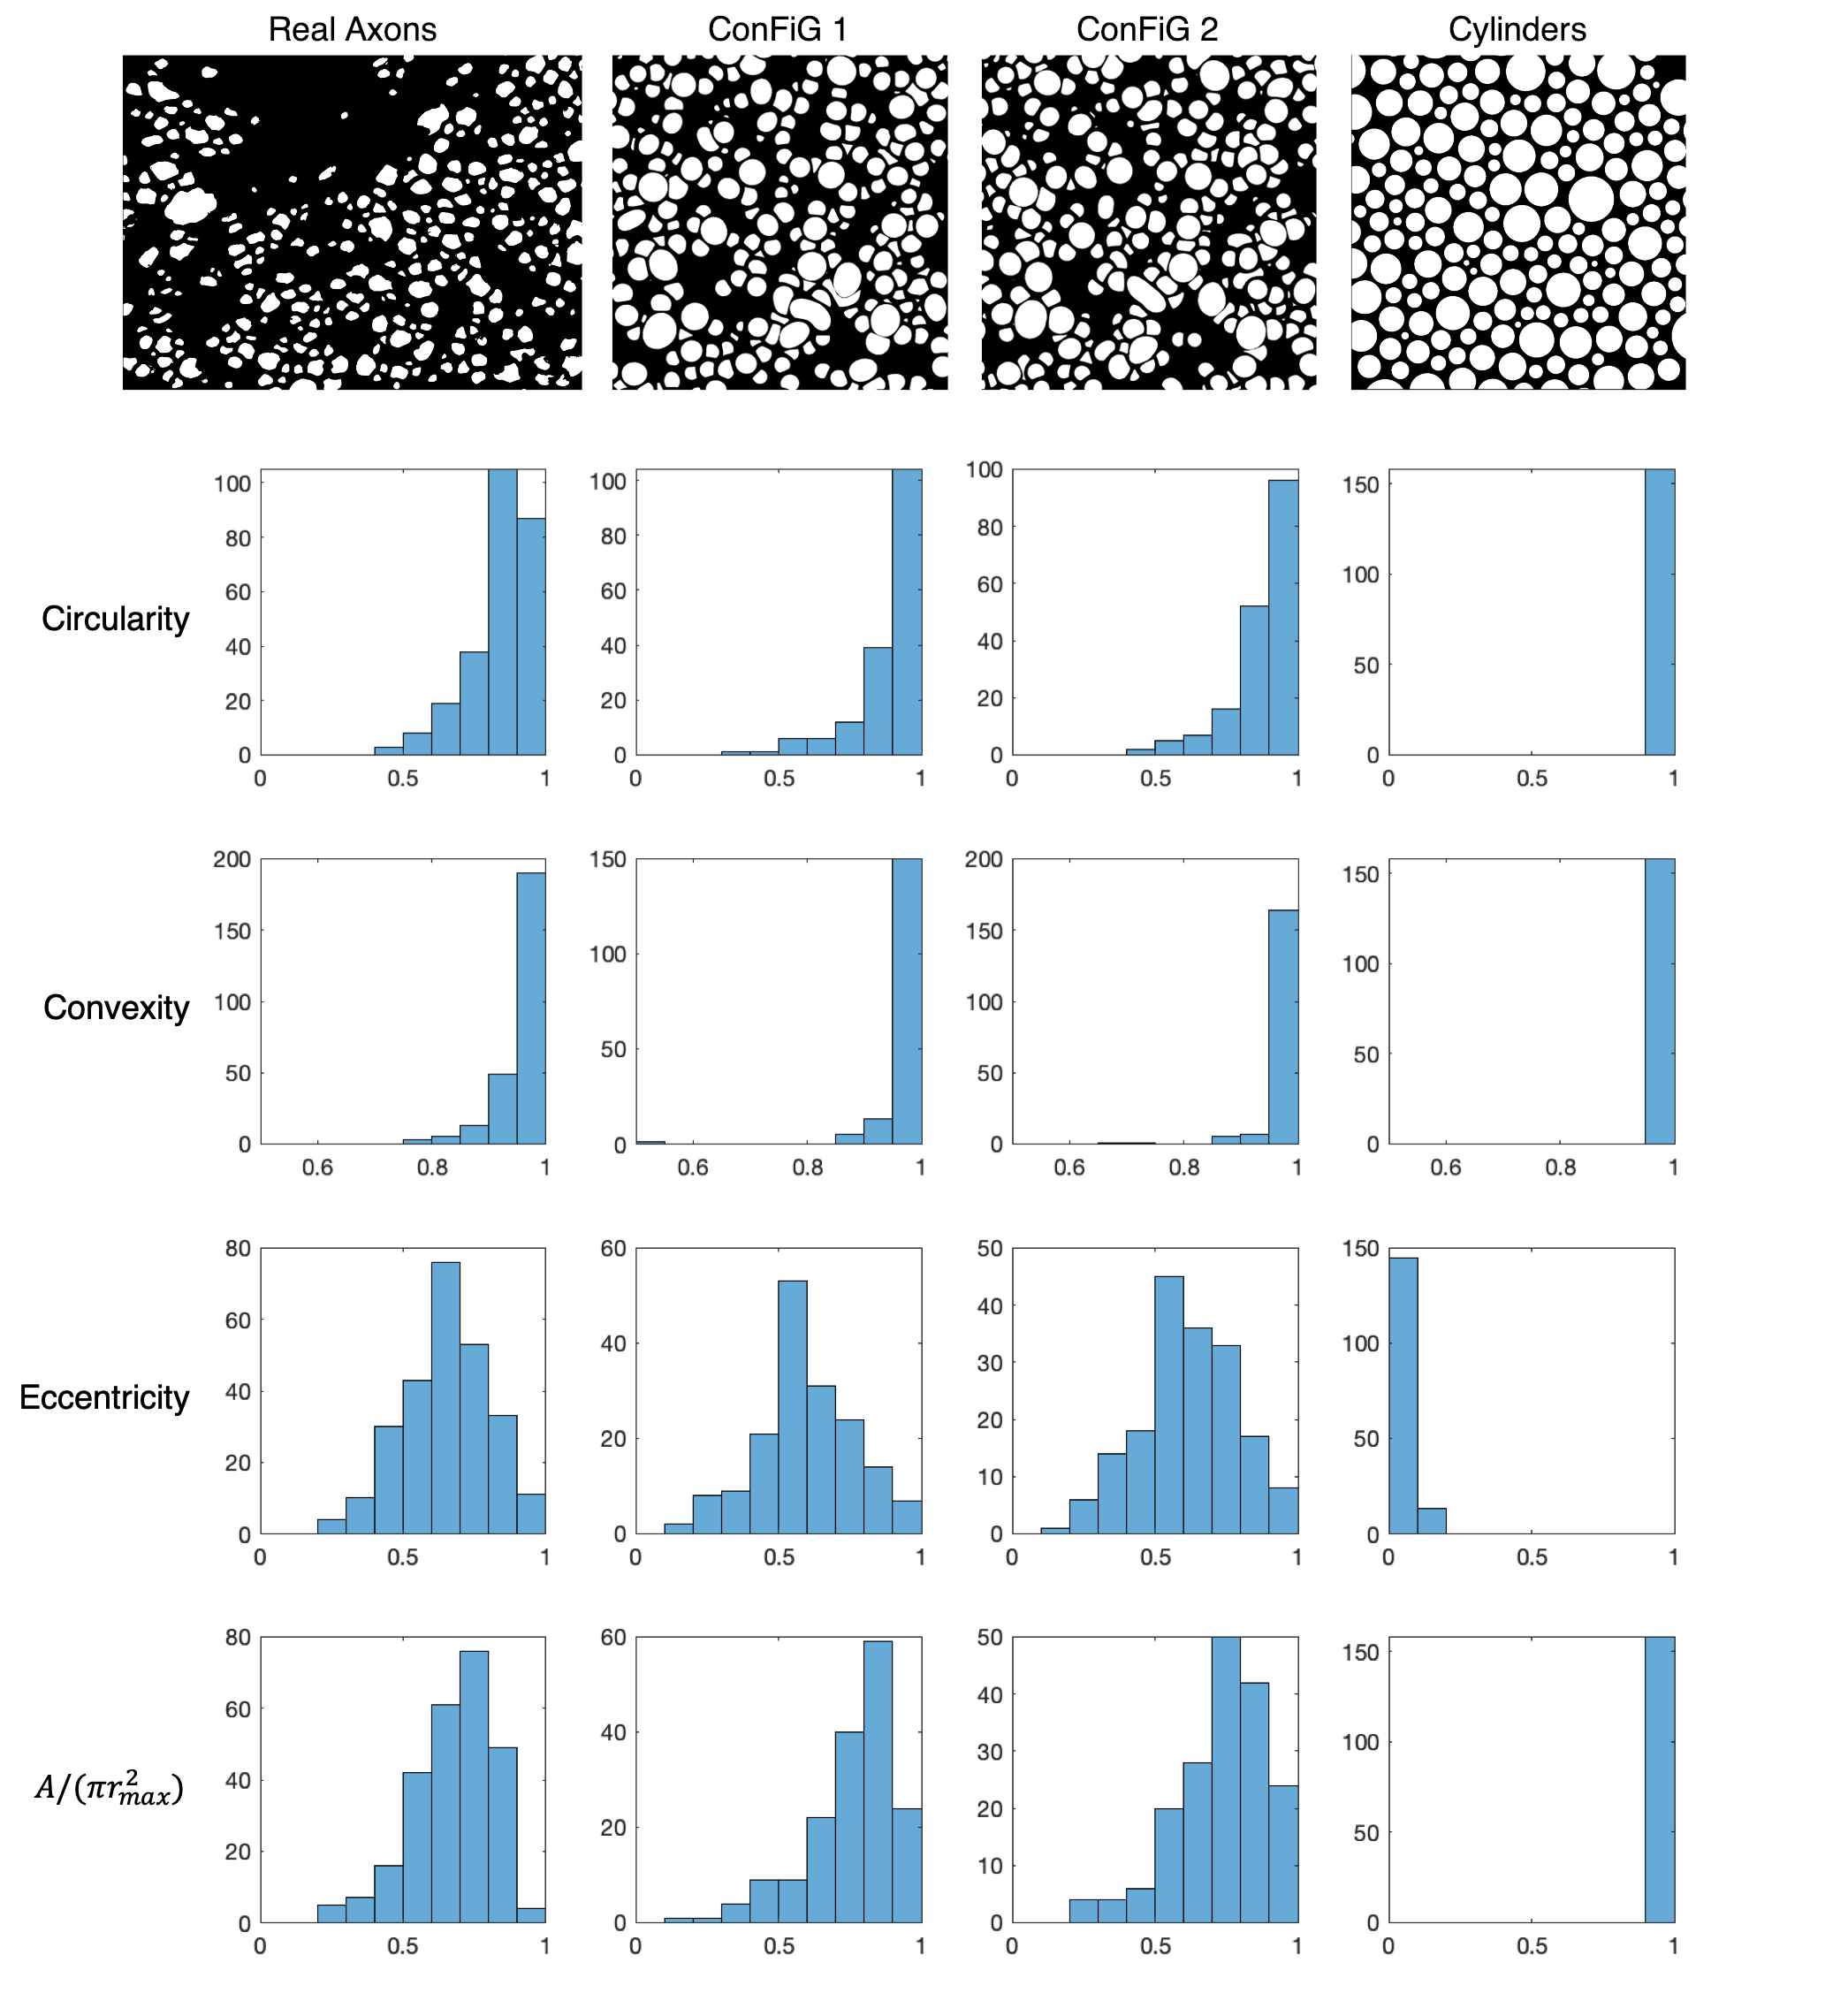
\includegraphics[width=\textwidth]{figures/config/slice_wise_metrics_whitebg.png}
  \caption[Slice-wise microstructural measurements]{Slice wise morphological metrics calculated for real axons, \ac{ConFiG} phantoms and parallel cylinders. Across each of the metrics, \ac{ConFiG} produces much more realistic distributions than  the cylinder phantom. Some of the cylinders have a non-zero eccentricity, but this arises since the metrics are calculated from binary images where the pixelated circles may appear to not be perfectly circular.}
  \label{fig:config_res_slice_wise_metrics}
\end{figure}

\begin{figure}
  \centering
  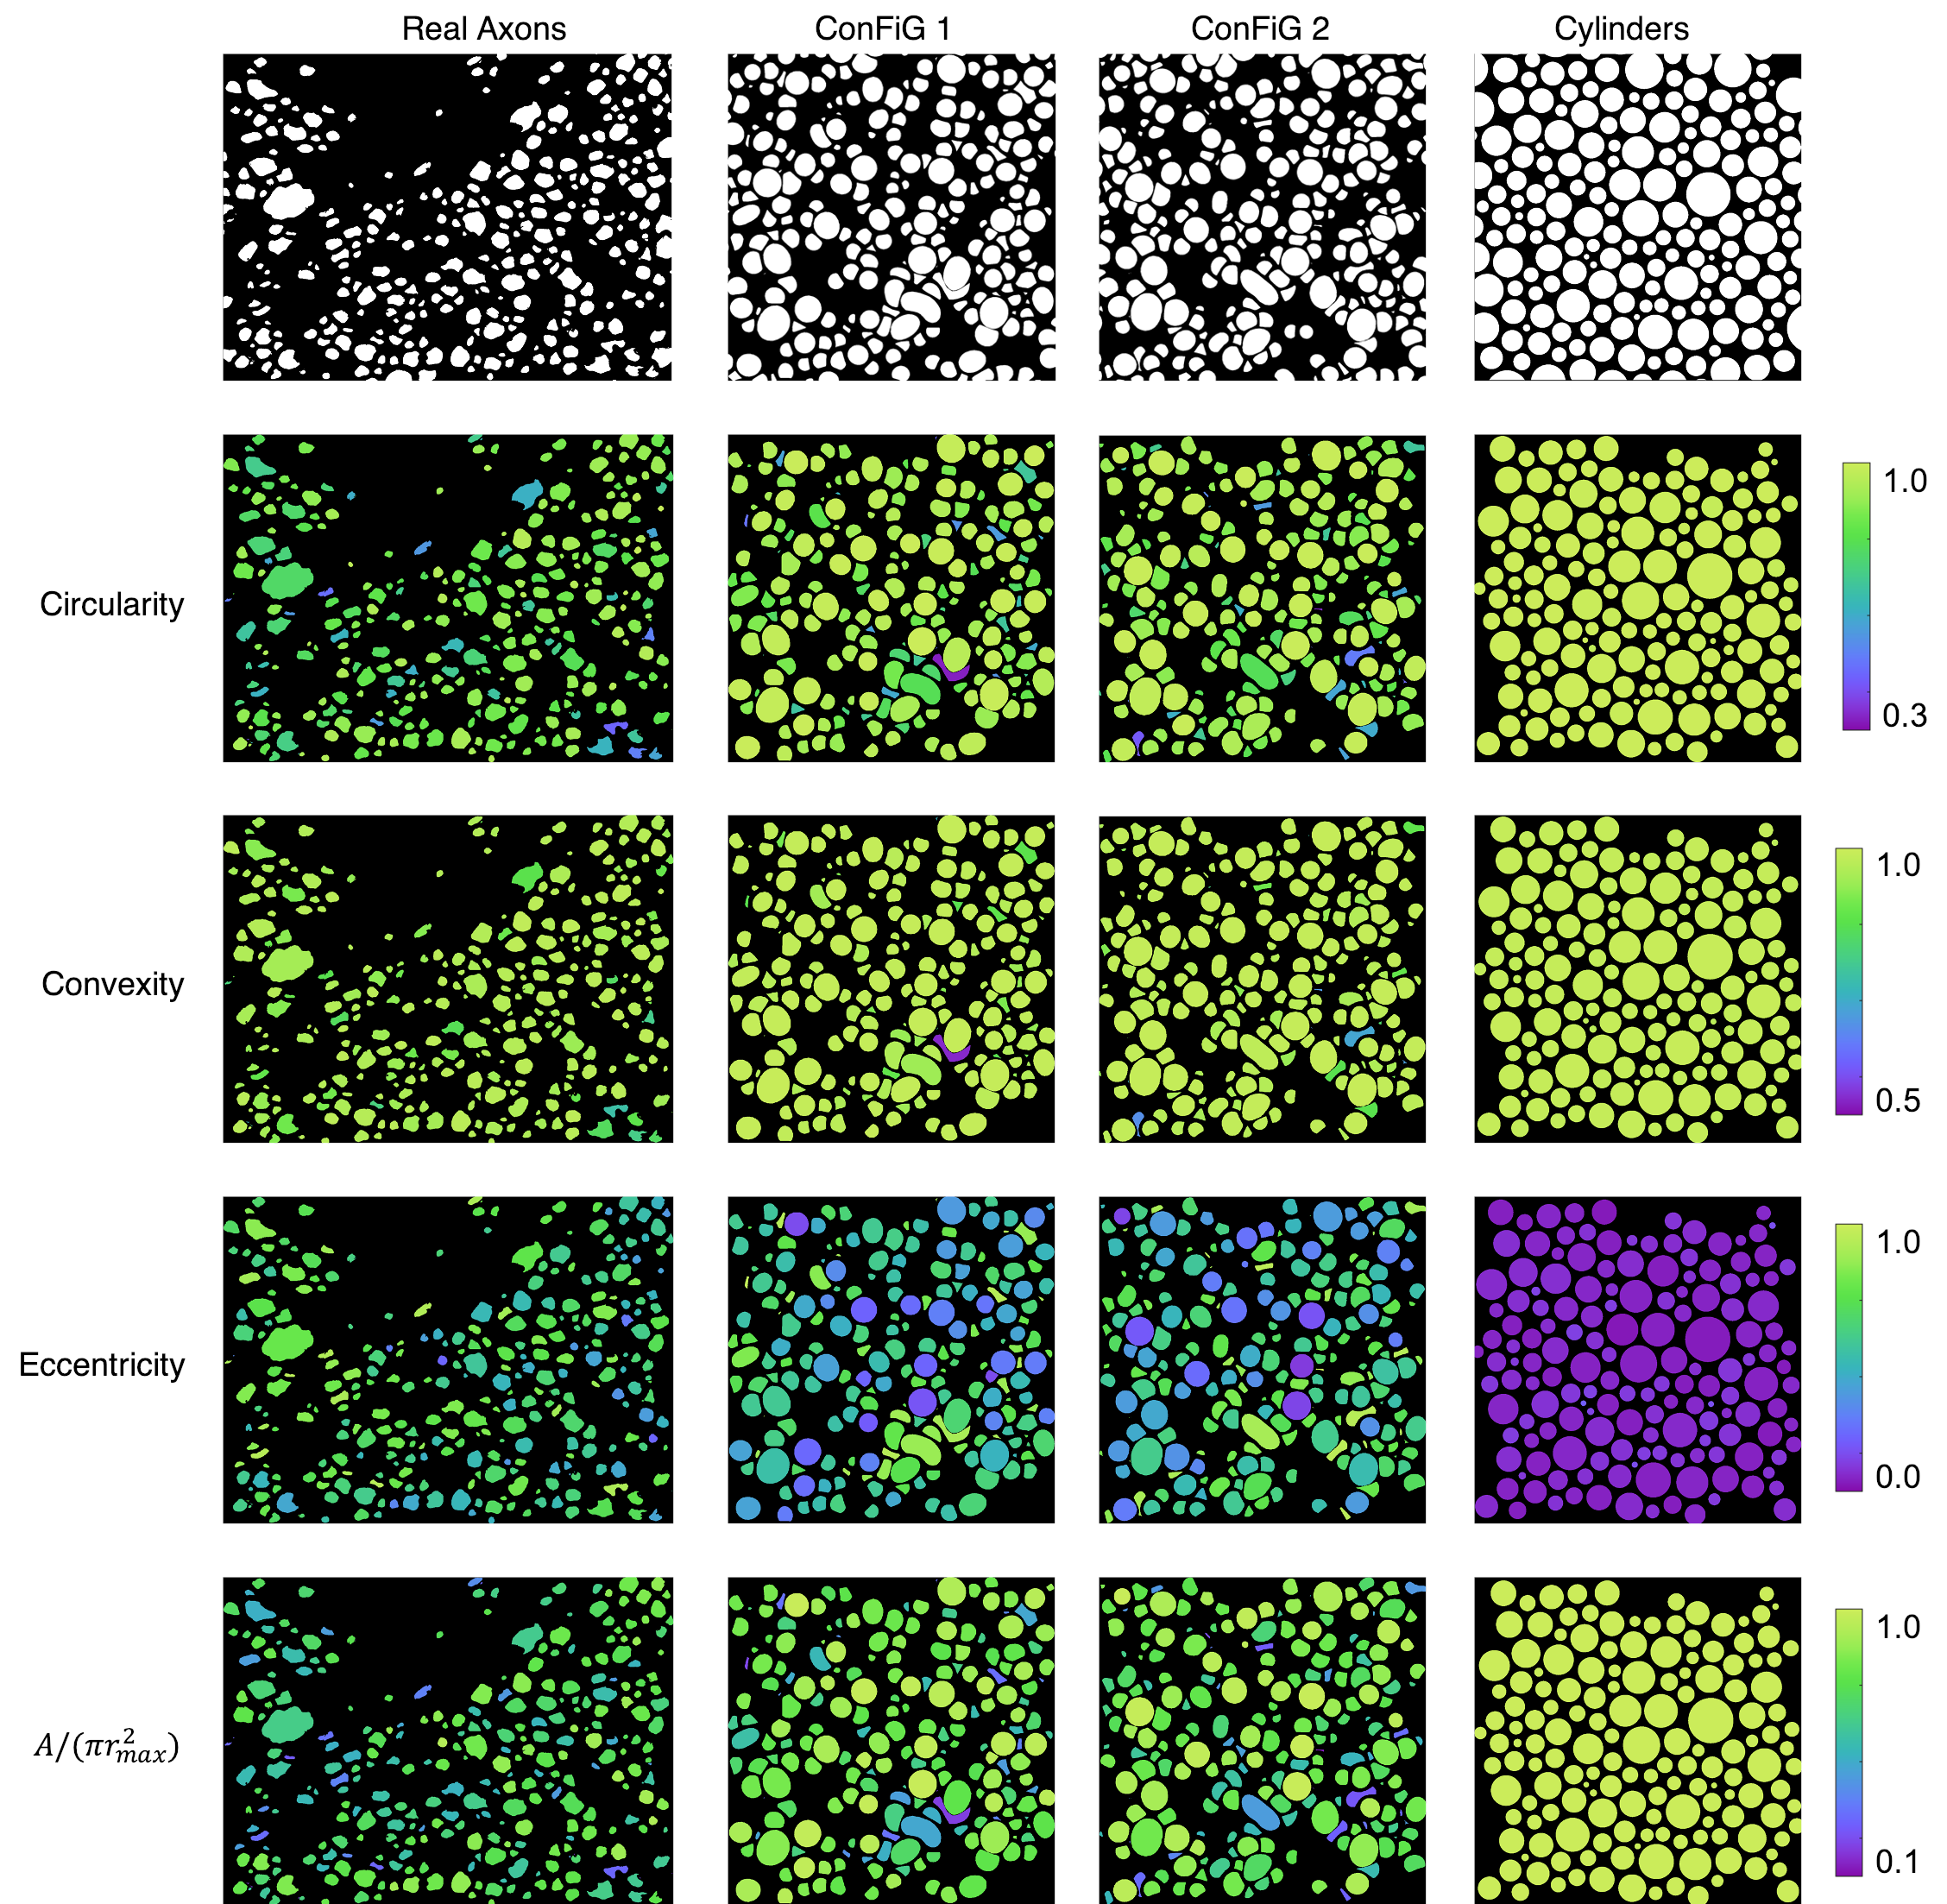
\includegraphics[width=\textwidth]{figures/micro/slice_wise_metrics_colormap_whitebg}
  \caption[Slice-wise microstructural measurements with colormap]{Slice-wise microstructural measurements with colormap demonstrating which fibres are being picked out by which metrics. Again, this shows that the standard cylinder approach generates uniform cross-sections while nature produces much more variation which \ac{ConFiG} is much closer to capturing.}
  \label{fig:micro_slice_wise_colormap}
\end{figure}


\begin{figure}
  \centering
  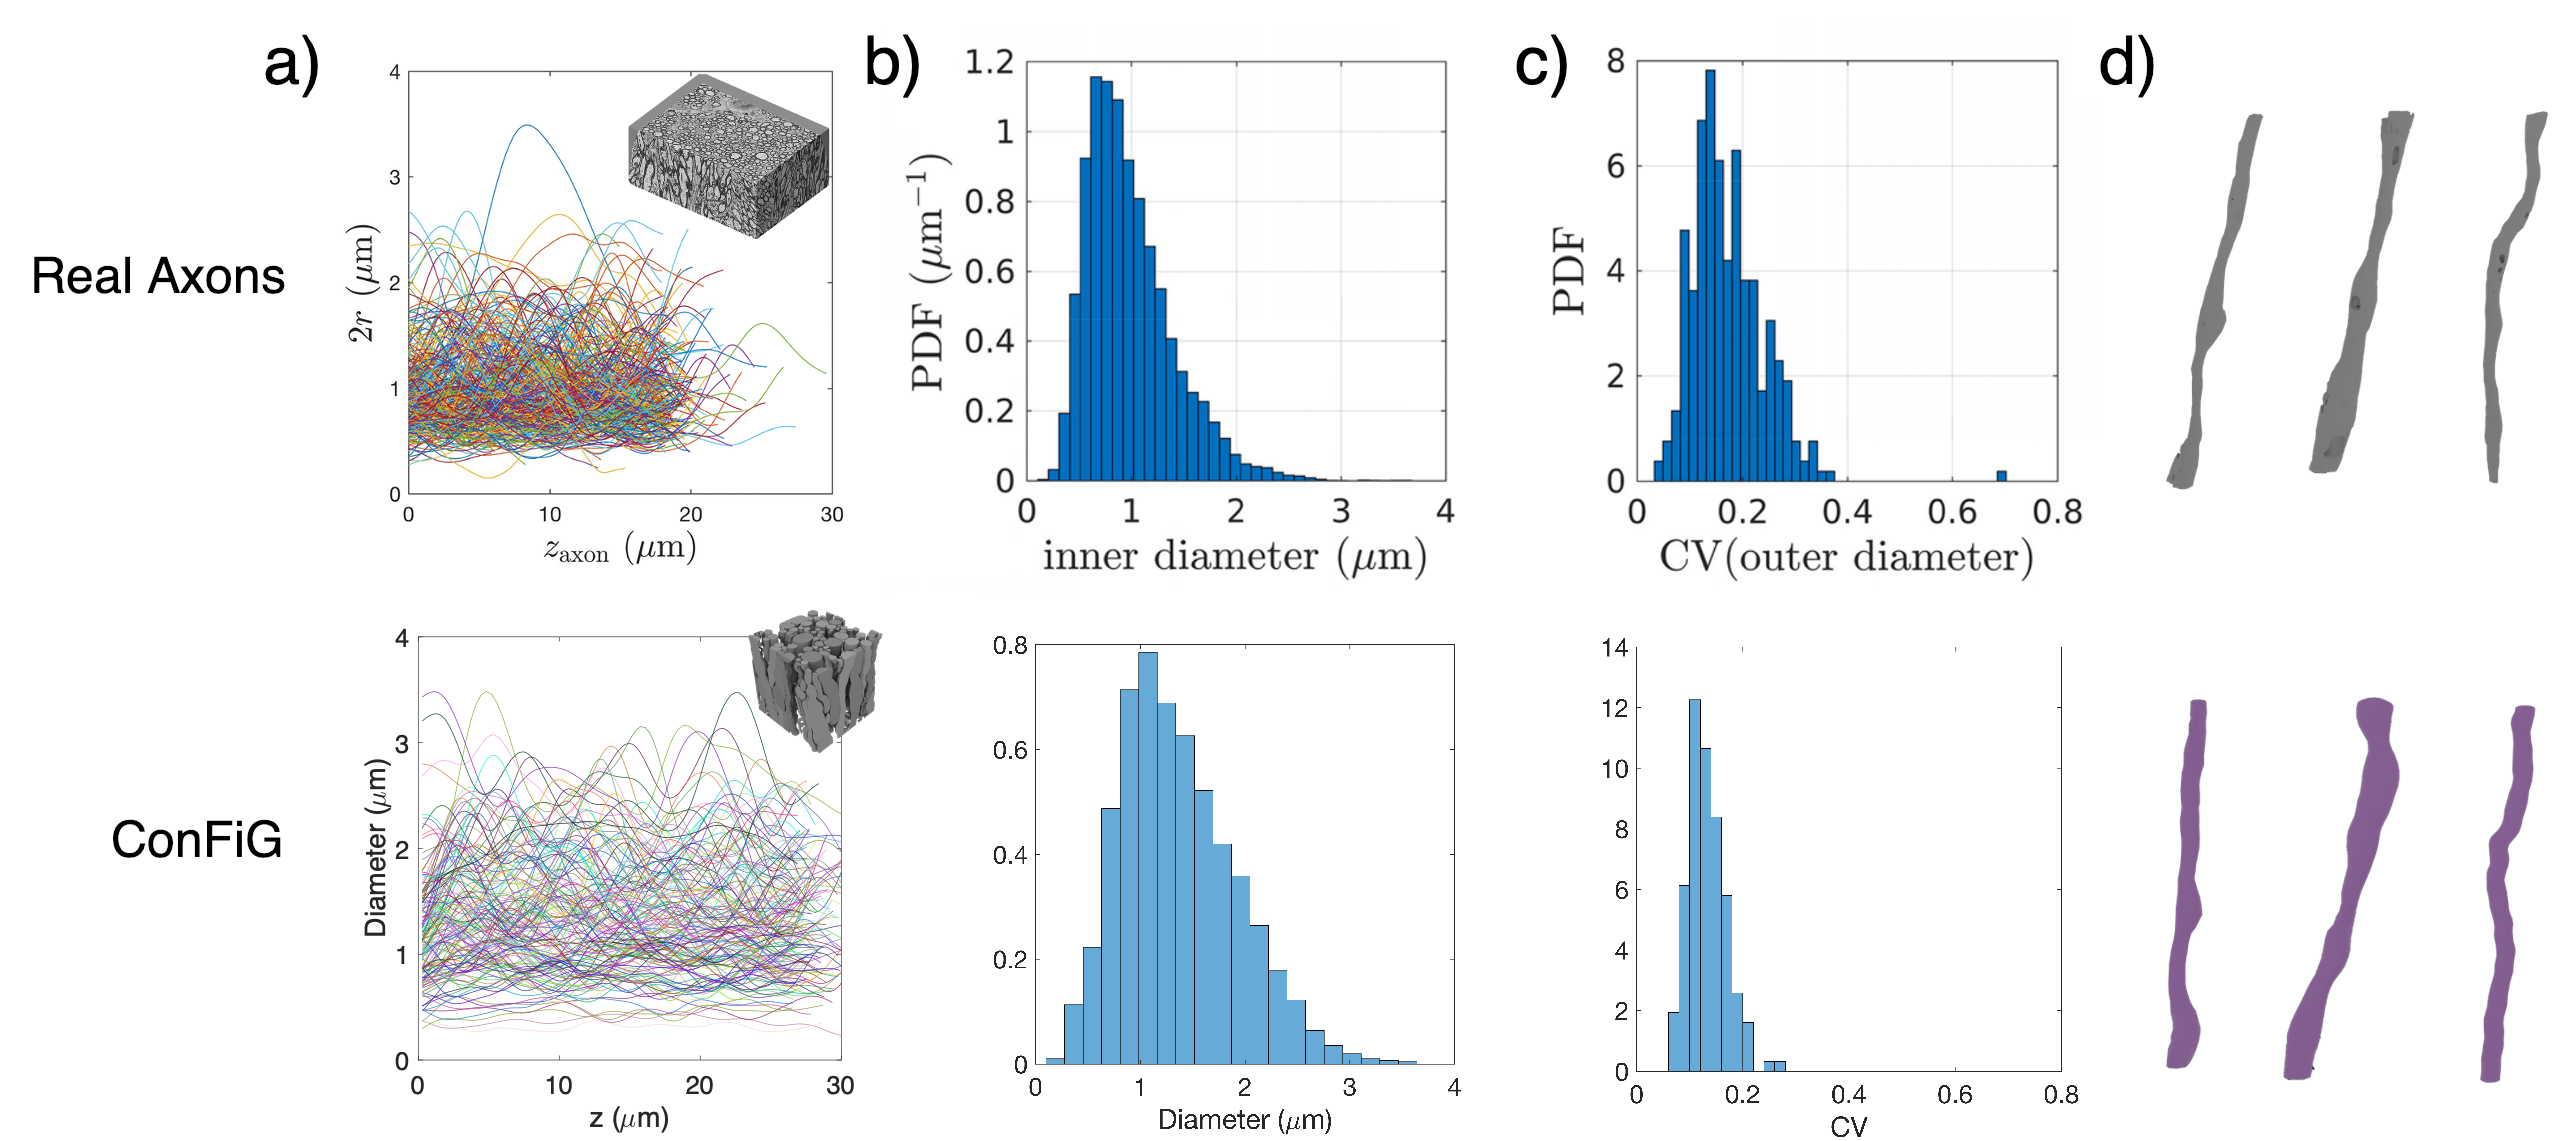
\includegraphics[width=\textwidth]{figures/config/diameter_dist_NEW_whitebg.png}
  \caption[Diameter distributions of real and \ac{ConFiG} axons]{a) Along fibre diameter variation in ex vivo mouse corpus callosum, reproduced from Lee et al. \cite{Lee2019b} compared to along axis diameter variation in the phantom inset demonstrating the ability of \ac{ConFiG} to generate realistic microstructure. b) Histograms of the inner diameter of axons from Lee et al. \cite{Lee2019b} and diameter of \ac{ConFiG} axons. c) Coefficient of variation along axons for real and \ac{ConFiG} axons and d) Three example fibres reconstructed from the \ac{EM} data used by Lee et al. to make a). d) Three example \ac{ConFiG} fibres selected for similarity to the \ac{EM} examples }
  \label{fig:config_res_diameter_dist}
\end{figure}

The diameter distribution of a \ac{ConFiG} substrate is compared to a reconstruction from real \ac{EM} data \cite{Lee2019b} in \Cref{fig:config_res_diameter_dist}. \ac{ConFiG} is able to capture the general profile of axonal variations well, with the overall shape of the diameter distribution matching well. The distribution of the coefficient of variation along \ac{ConFiG} axons is slightly narrower with a smaller mean than real axons, though these discrepancies may be alleviated with a different choice of input parameters to \ac{ConFiG}.

\ac{ConFiG} is also able to generate \acp{FOD} comparable to real tissue as shown in \Cref{fig:config_res_OD}. Here the fibre paths are smoothed with a Gaussian kernel equivalent to having a diffusion time of \SI{1}{\milli\second} and diffusivity of \SI{2}{\micro\metre\squared\per\milli\second} as in Lee et al.\ \cite{Lee2019b}. The orientation dispersion is introduced to \ac{ConFiG} phantoms using the \acf{ESAG}~\cite{Paine2018} to best approximate the \ac{EM} data and also using isotropic Watson distributed directions to demonstrate the flexibility of \ac{ConFiG}.


\begin{figure}
  \centering
  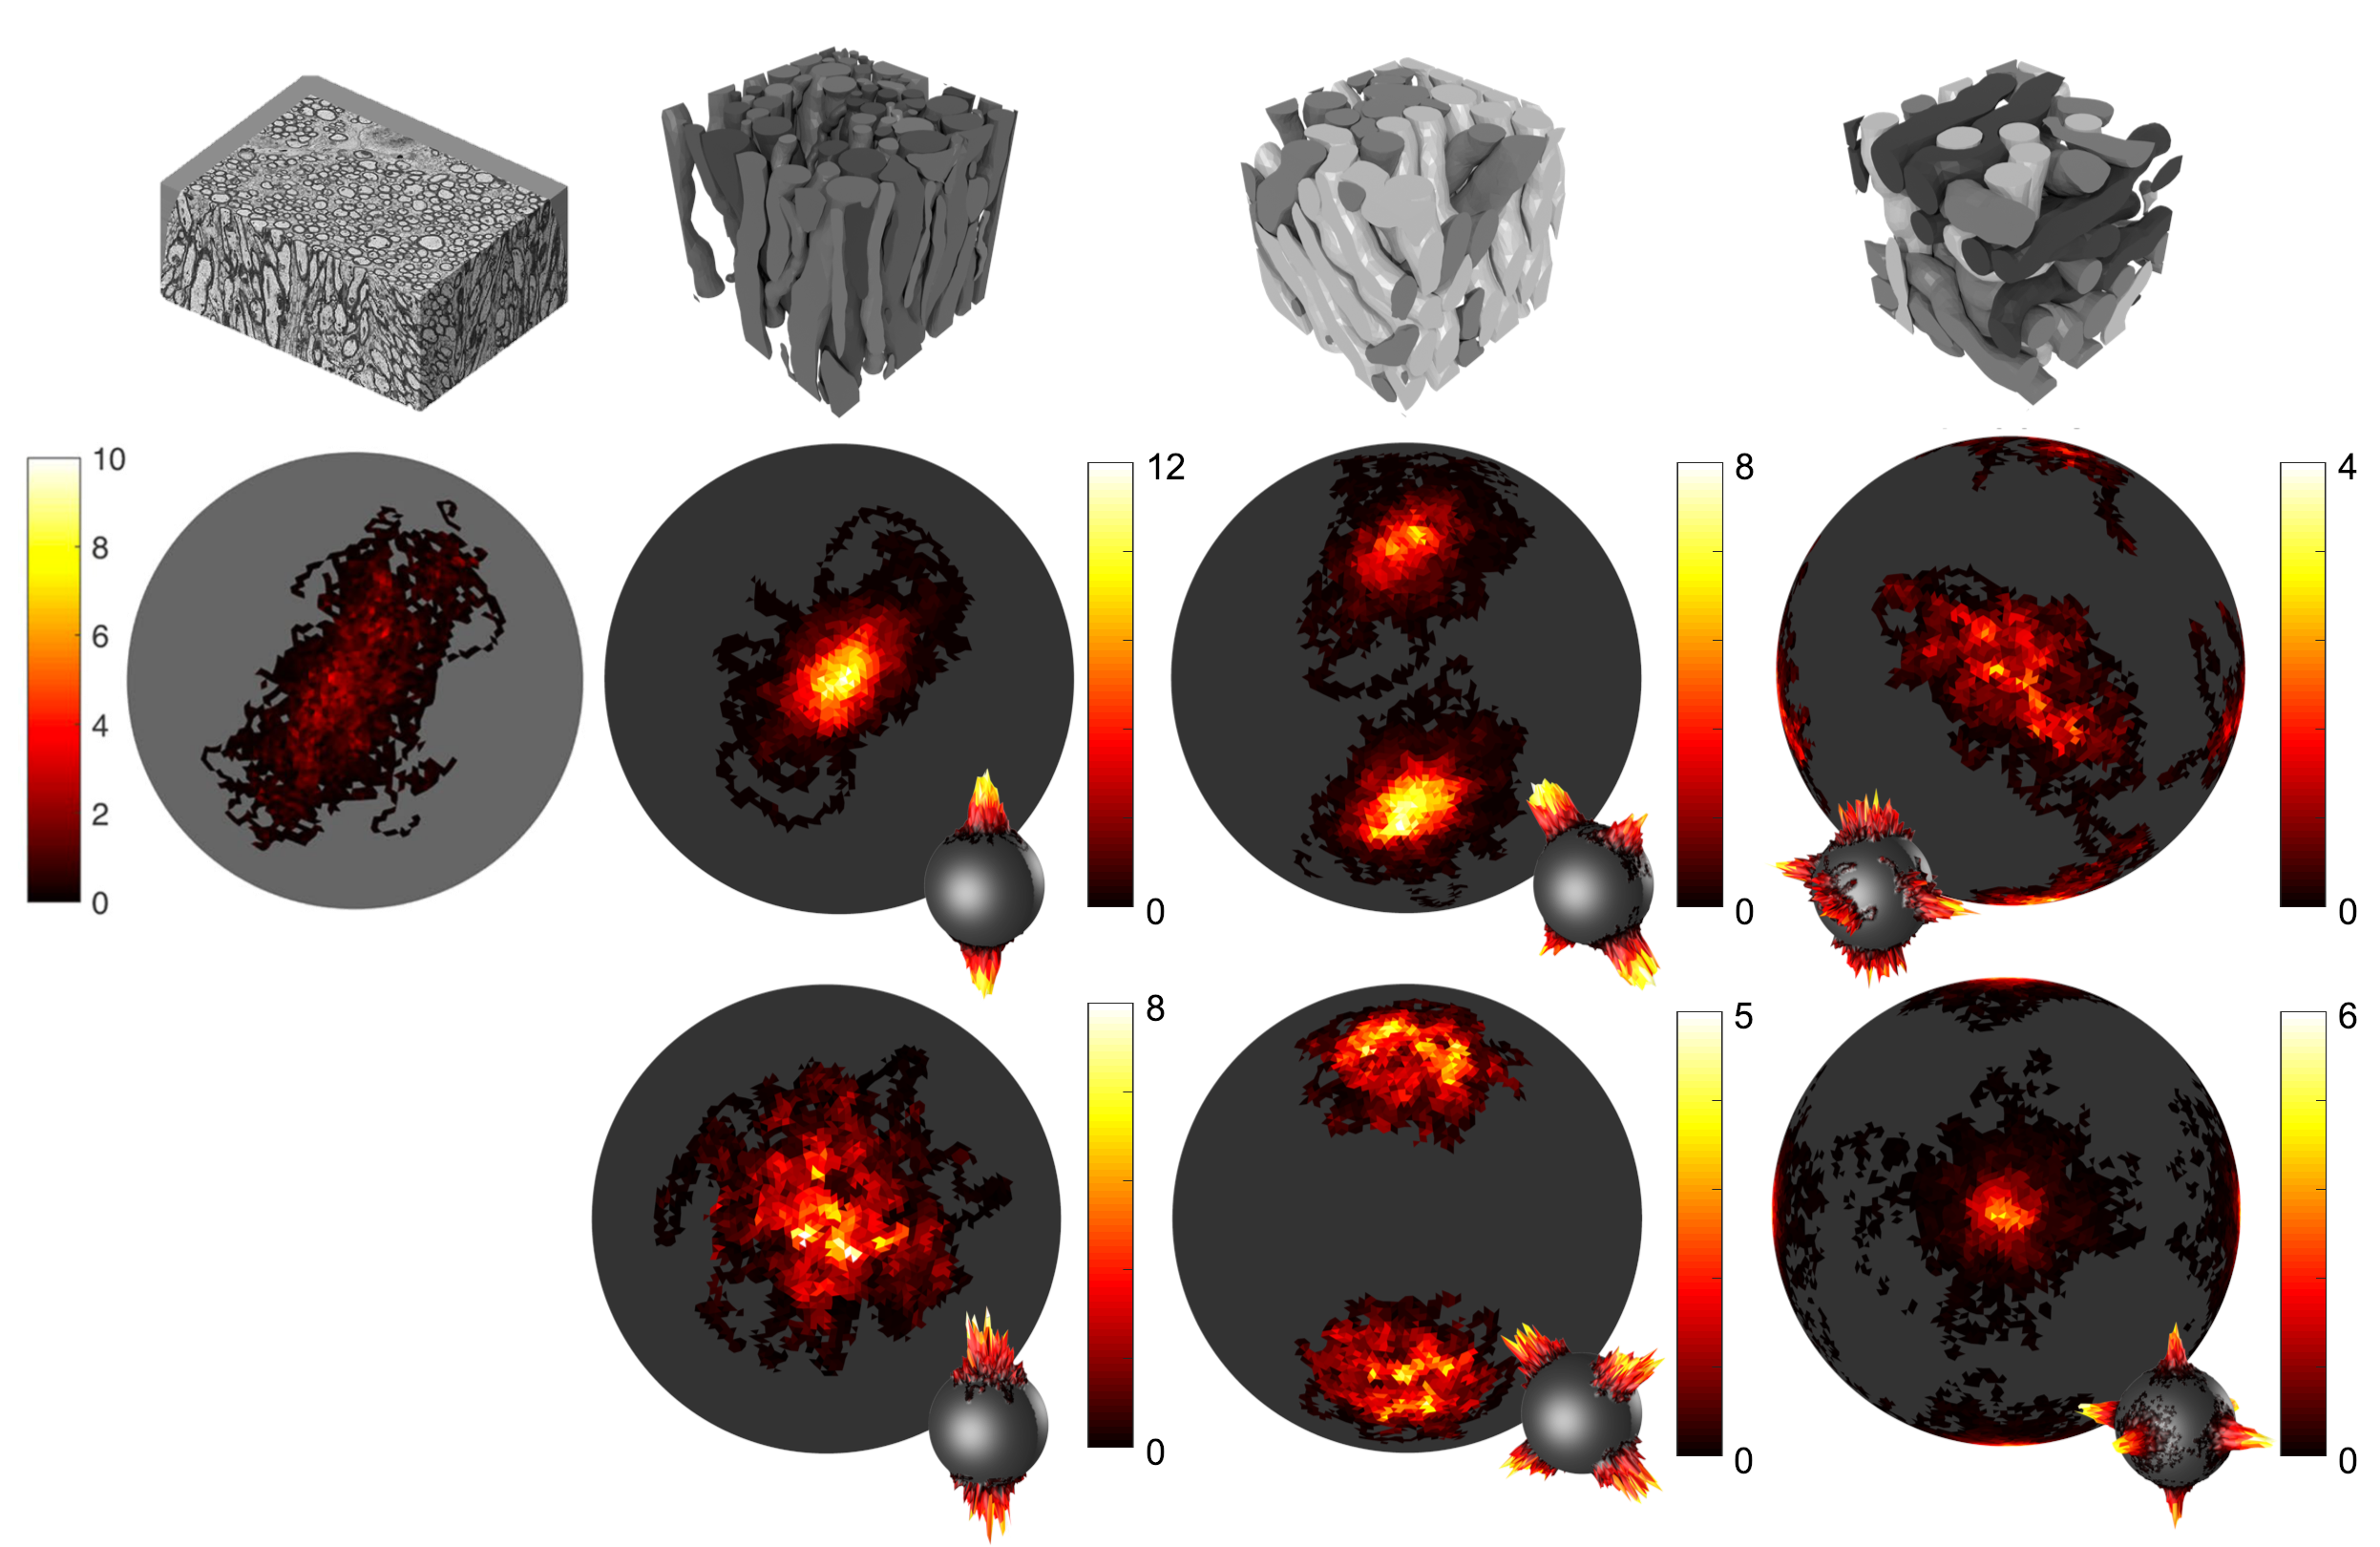
\includegraphics[width=\textwidth]{figures/config/OD_ESAG_wcolorbar_wiso_sym_whitebg.png}
  \caption[Orientation distributions from real WM and \ac{ConFiG} phantoms]{Fibre orientation distributions for \ac{EM} data and a series of numerical phantoms. Top row: \ac{EM} data used to generate \ac{FOD}, reproduced from Lee et al. \cite{Lee2019b} and three \ac{ConFiG} phantoms with one, two and three crossing bundles (each crossing bundle coloured a different shade of grey). Middle row: \ac{FOD} profile for real \ac{EM} data and \ac{FOD} profiles corresponding to \ac{ConFiG} phantoms above, generated using an elliptically symmetric dispersion. Bottom row: Three \ac{FOD} profiles generated from \ac{ConFiG} phantoms generated using isotropic orientation dispersion. Colormap has units of \si{\per\steradian}. }
  \label{fig:config_res_OD}
\end{figure}

\subsection{Relationship between input and output morphology}
\label{sec:config_result_input_output_rel}
\begin{table}[]
\caption{Comparison between input microstructural parameters and the microstructure measured in the resulting \ac{ConFiG} phantoms. For each phantom, an input target density, $\rho$, of 75\% was used with each phantom having a different value of $\kappa$ used in the Watson distribution. Each $\kappa$ is associated with a target $\mu_\theta$ and $\sigma_\theta$, the mean and standard deviation of the angle away from the main bundle direction. Angles reported in degrees.}
\label{tab:micro_input_vs_output}
\begin{tabular}{ccccccc}
  \toprule
  Input $\kappa$ & Input $\rho$ & Output $\rho$ & Target $\mu_\theta$ & Output $\mu_\theta$ & Target $\sigma_\theta$ & Output $\sigma_\theta$\\\midrule
8        & 75\%     & 70.6\%    & 19.60     & 17.46     & 11.32     & 9.92   \\
10       & 75\%     & 73.4\%    & 17.11     & 16.47     & 9.62      & 9.43   \\
15       & 75\%     & 73.4\%    & 13.60     & 13.93     & 7.37      & 8.75   \\
20       & 75\%     & 70.7\%    & 11.68     & 12.69     & 6.23      & 7.88   \\
30       & 75\%     & 72.0\%    & 9.45      & 11.60     & 5.02      & 6.60   \\
50       & 75\%     & 73.6\%    & 7.26      & 9.36      & 3.83      & 5.51   \\
100      & 75\%     & 74.9\%    & 5.10      & 7.75      & 2.68      & 4.23 \\\bottomrule
\end{tabular}
\end{table}

The morphology of \ac{ConFiG} phantoms matches the input morphology well, as shown in \Cref{tab:micro_input_vs_output}. Whilst the input and output $\mu_\theta$ and $\sigma_\theta$, do not match exactly, the values are close and increasing the input $\mu_\theta$ and $\sigma_\theta$ also increases the output $\mu_\theta$ and $\sigma_\theta$. Additionally, the output density generally matches the input target density well, achieving higher densities than MEDUSA for the same angular dispersion.
%Supplementary Table 1 shows the same experiment run with a target density of 60\% to demonstrate \ac{ConFiG}’s performance at lower densities.

These phantoms took an average of 6 hours to grow plus an average of 20 minutes for the meshing and microstructural measurement procedure, using 9.4GB of RAM on average. These values give an estimate of the time taken to generate a typical \ac{ConFiG} phantom, though it is strongly dependent on user inputs (number of nodes in the network etc.).

\subsection{Packing induced microsctructural complexity}
\label{sec:micro_res_packing}
The more complex the fibre orientation in a phantom, the more complex the microstructure that is generated will be as demonstrated in \Cref{fig:micro_packing_induced_complexity}.
Both the mean tortuosity and mean coefficient of variation grow as more orientation dispersion is introduced to the phantom (\Cref{fig:micro_packing_induced_complexity}a\&b), with the two showing a positive correlation (\Cref{fig:micro_packing_induced_complexity}).


\begin{figure}
  \centering
  \begin{subfigure}[]{0.32\textwidth}
    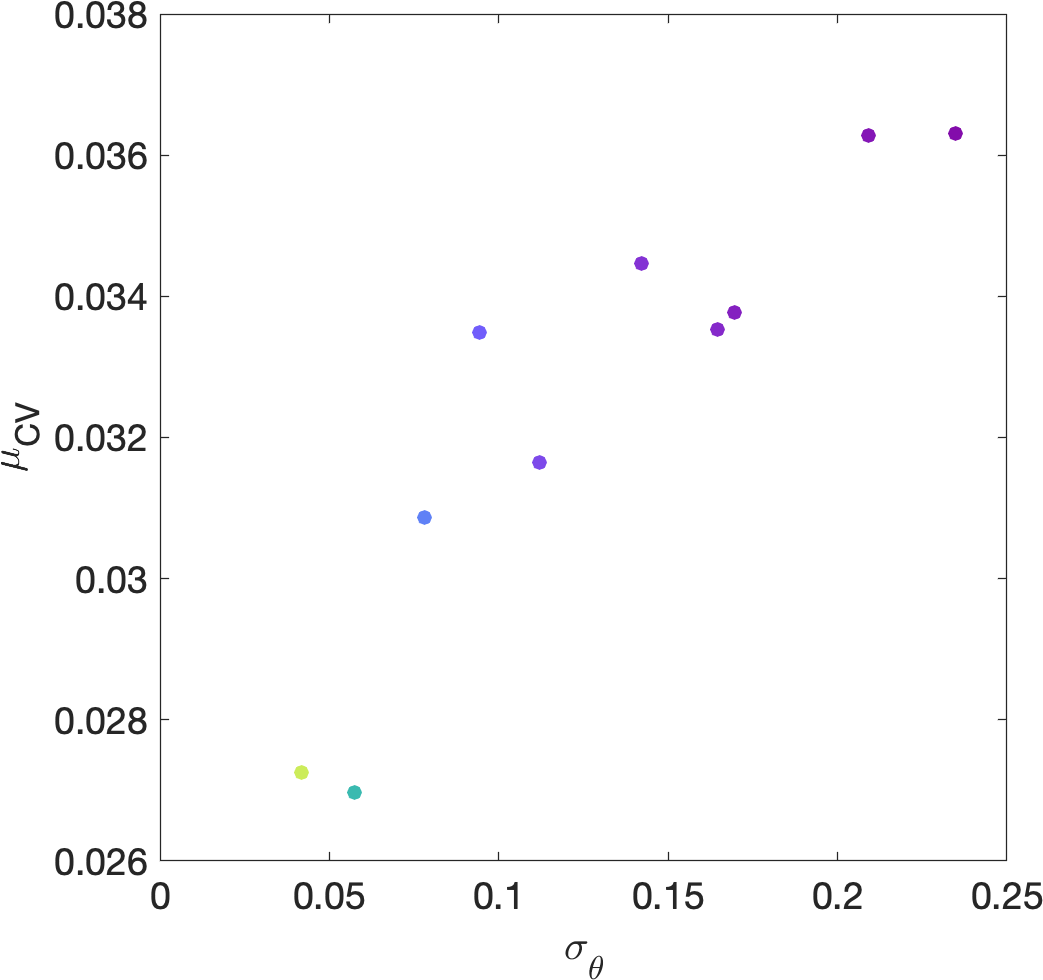
\includegraphics[width=\textwidth]{figures/micro/meanCV_vd_std_theta}
    \caption{}
  \end{subfigure}
  ~
  \begin{subfigure}[]{0.32\textwidth}
    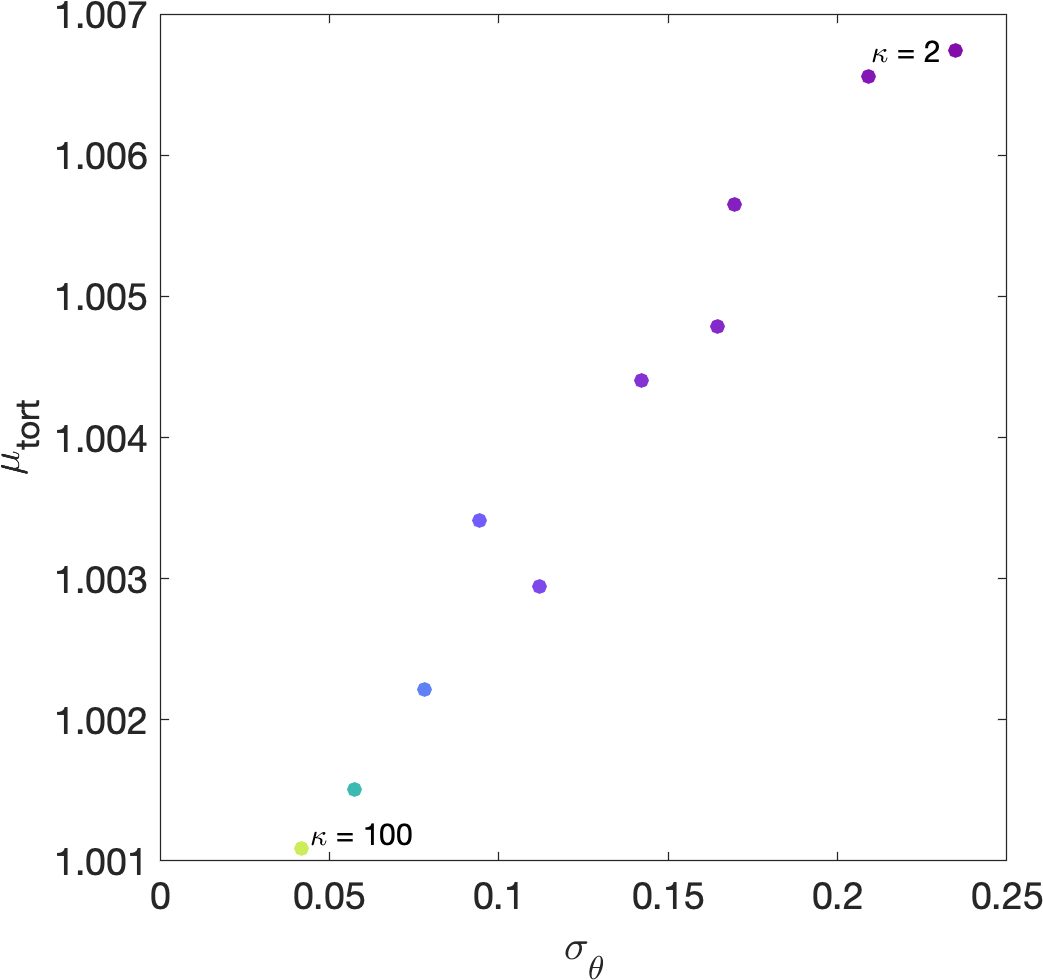
\includegraphics[width=\textwidth]{figures/micro/meantort_vd_std_theta}
    \caption{}
  \end{subfigure}
  ~
  \begin{subfigure}[]{0.32\textwidth}
    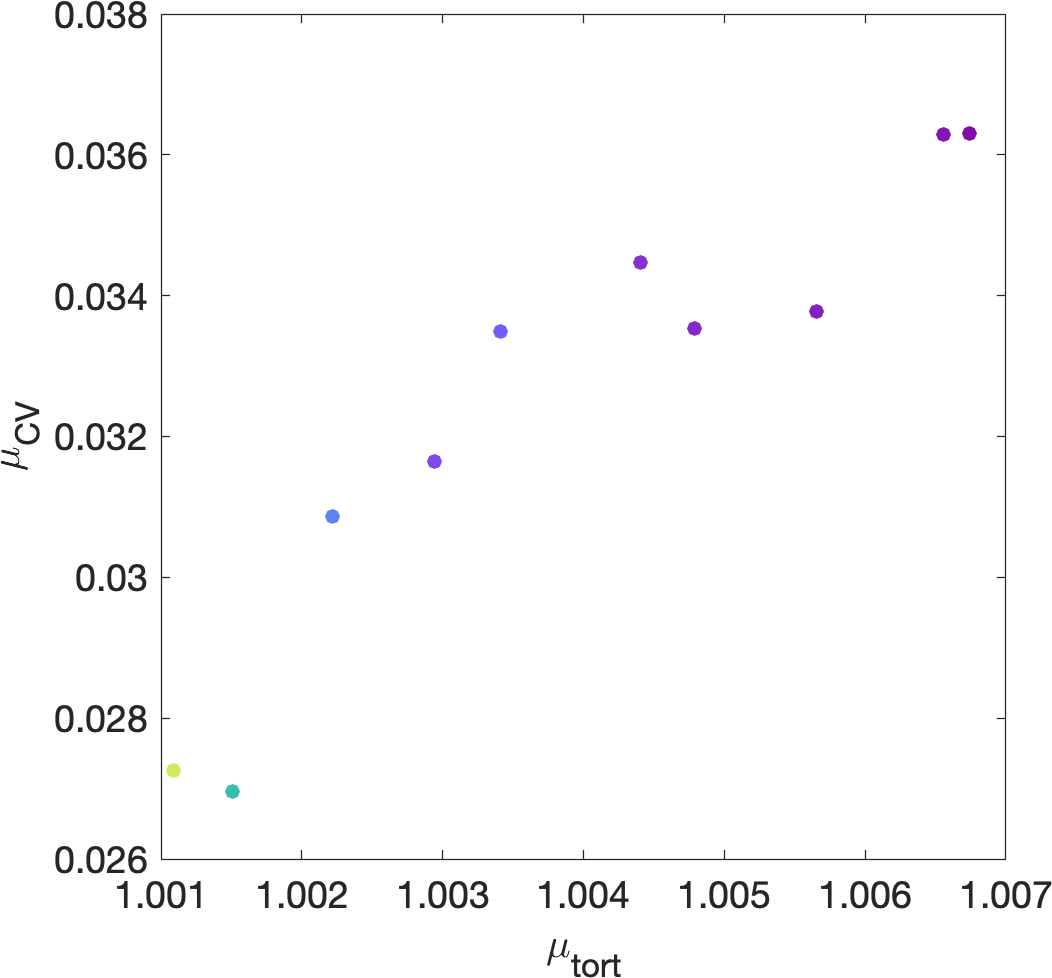
\includegraphics[width=\textwidth]{figures/micro/meantort_vd_meanCV}
    \caption{}
  \end{subfigure}
  \caption[Packing induced microstructural complexity]{Packing induced microstructural complexity. (a) the mean coefficient of variation in a phantom ($\mu_{\mathrm{CV}}$) grows with increased orientation dispersion in the phantom, as does (b) the mean tortuosity ($\mu_{\mathrm{tort}}$). (c) $\mu_{\mathrm{tort}}$ and $\mu_{\mathrm{CV}}$ are positively correlated showing that for \ac{ConFiG} phantoms, complex arrangements of fibres are achieved through both undulation and beading of fibres. }
  \label{fig:micro_packing_induced_complexity}
\end{figure}




\section{Discussion}
\label{sec:micro_discussion}

\ac{ConFiG} is shown to produce realistic WM numerical phantoms, capturing microscopic structural features such as diameter and orientation distributions. The amount of real data containing 3D microstructural morphology information available to compare to is limited, so we have only compared to one sample in this study. Whilst limited, this shows that \ac{ConFiG} is able to produce realistic microstructure by following simple biologically inspired growth rules.

\Cref{fig:config_res_slice_wise_metrics,fig:micro_slice_wise_colormap} demonstrates that \ac{ConFiG} phantoms are able to create fibre morphologies that match real axons much more closely than previous methods based on cylinders. Whilst some of the features such as eccentricity may be achievable with cylinders oriented obliquely to the cutting plane, \ac{ConFiG} phantoms capture morphological features that are otherwise impossible with cylinders such as convexity less than one.

Whilst the input morphological priors do not necessarily correspond to the morphology of the resulting \ac{ConFiG} phantom, \Cref{tab:micro_input_vs_output} shows that even for relatively high orientation dispersion and density, this effect is small. Even so, for use in further analysis, microstructural measures such as orientation dispersion and density should be calculated based on the resultant phantom, rather than taking the input microstructural parameters.

Related to this effect, \Cref{fig:micro_packing_induced_complexity} shows that as the input fibre orientation becomes more complex, with increased \ac{OD}, the microstructural complexity increases. Both the tortuosity in the fibre paths and the coefficient of variation in diameter along fibres grows with increased \ac{OD} in the phantom. 

\subsection{Limitations and future Work}
\label{sec:micro_limitations}

As mentioned above, this study only compares \ac{ConFiG} to one \ac{EM} sample of real tissue. Future work will also aim at more extensive validation of the digital phantoms generated using \ac{ConFiG}, making comparison with larger \ac{EM} datasets, including different WM configurations from different brain regions.

One limitation of this and future work is ambiguity in the definition of the \acp{FOD} which are displayed in \Cref{fig:config_res_OD}.
In this work, since we're concerned with the actual microstructure of the phantoms we calculate the \ac{FOD} with a small amount of smoothing to compare with Lee et. al \cite{Lee2019b}.
One consequence of this `microscopic' definition of the \ac{FOD} is that individual fibres contribute to more than one direction in the distribution (this can be seen in \Cref{fig:config_res_OD} with the loops on the edges of the distributions which come from individual fibres). 
This is contrary to the \ac{FOD} more commonly used in \ac{dMRI} techniques such as tractography \cite{DellAcqua2019,Schilling2019b,Tournier2007,Tournier2004} which assumes each fibre contributes to a single direction only. 
It remains to be seen how these two definitions of the \ac{FOD} can be brought together, thought it would certainly be a valuable contribution to be able to test the performance of \ac{FOD} estimation techniques to the `true' microscopic \ac{FOD}. 

We will work towards decreasing the difference between the input and output morphological measures, particularly in complex situations, such as high orientation dispersion and crossing bundles. This can be addressed through the improvements to \ac{ConFiG} mentioned in \Cref{sec:config_conclusion} and also by improving the strategy for the generation of starting and target points for each fibre. For instance, currently it is not intuitive how starting and target points should be arranged to achieve a desired density in crossing regions of fibres.


\section{Conclusion}
\label{sec:micro_conclusion}
The experiments presented here demonstrate the microscopic realism of \ac{ConFiG} phantoms. Microstructural measurement methods have been developed which enable the quantification of axonal microstructure from \ac{ConFiG} meshes and are used to demonstrate that \ac{ConFiG} captures axonal diameter and orientation distributions that agree well with real axonal microstructure.
Not only that, but \ac{ConFiG} captures subtle, complex features such as bulges and non-circular cross-sections bringing \ac{WM} phantoms much closer to real tissue than the previous standard of cylinders.
Whilst only comparing to a single tissue sample, these experiments give us confidence that the microstructure generated using \ac{ConFiG} is a big step forwards towards realistic \ac{WM} numerical phantoms. 


%%% Local Variables:
%%% mode: latex
%%% TeX-master: "../main"
%%% End:
